\documentclass[10pt]{article}

\usepackage[utf8]{inputenc}
\usepackage[a4paper, total={6in, 8in}]{geometry}
\usepackage{graphicx}
\usepackage{indentfirst}
\usepackage{hyperref}
\usepackage{amsmath}
\usepackage{amssymb}
\usepackage{tikz}
\usetikzlibrary{calc,intersections}

\newcommand{\figuresize}{8cm}
\newcommand{\degreecolor}{green!20!white}
\newcommand{\degreebordercolor}{green!50!black}
\newcommand{\degree}{^{\circ}}
\newcommand{\makeangle}[7]{
	\begin{scope}
	\path[clip] (#2) -- (#1) -- (#3);
	\fill[green!20!white, draw=green!50!black] (#2) circle (#5);
	\node at ($(#2)+(#6:#7)$) {$#4^{\circ}$};
	\end{scope}
}

\begin{document}

	\begin{titlepage}

        \title{Geometry for fun}
        \author{Henrique Tsuyoshi Yara}
        \date{\today}

        \null  % Empty line
        \nointerlineskip  % No skip for prev line
        \vfill
        \let\snewpage \newpage
        \let\newpage \relax

        \maketitle

        \vspace{1in}
        \begin{figure}
            \centering
            
\includegraphics[width=5cm]{my_avatar}
            \caption{My avatar :D}
        \end{figure}

        \thispagestyle{empty}
        \let \newpage \snewpage
        \vfill
        \break % page break

    \end{titlepage}

    \tableofcontents

    \section{Exercise 001}

\subsection{Problem}

\begin{figure}[ht]
	\centering
	\begin{tikzpicture}[x=\figuresize,y=\figuresize]
	\coordinate [label=below:$B$] (B) at (0,0);
	\coordinate [label=below right:$C$] (C) at (1,0);
	\coordinate [label=above:$D$] (D) at (0.03,0.17);
	\coordinate [label=above:$A$] (A) at (-0.27,1.51);
	\coordinate (CDmid) at ($(C)!0.5!(D)$);
	\coordinate (ACmid) at ($(A)!0.5!(C)$);

	\node at (CDmid)[above] {$a$};
	\node at (ACmid)[above right] {$2a$};
	
	\makeangle{D}{B}{C}{80}{0.08}{40}{0.12}
	\makeangle{B}{C}{D}{10}{0.12}{175}{0.30}
	\makeangle{A}{C}{D}{40}{0.08}{150}{0.12}
	\makeangle{B}{A}{C}{x}{0.08}{295}{0.12}

	\draw (B) -- (D) -- (C) -- (B) -- (A) -- (C);

	\end{tikzpicture}
	\caption{$\overline{DC} = a; \overline{AC} = 2a; \angle \hat{CBD} = 80\degree; \angle \hat{ACD} = 40\degree; \angle \hat{BCD} = 10\degree; \angle \hat{BAC} = ?$}
\end{figure}

\subsection{Solution 1}

\begin{figure}
	\centering
	\begin{tikzpicture}[x=\figuresize,y=\figuresize]
	\coordinate [label=below:$B$] (B) at (0,0);
	\coordinate [label=below right:$C$] (C) at (1,0);
	\coordinate [label=above left:$D$] (D) at (0.03,0.17);
	\coordinate [label=above:$A$] (A) at (-0.27,1.51);
	\coordinate [label=above:$E$] (E) at (0.36,0.76);
	\coordinate (AEmid) at ($(A)!0.5!(E)$);
	\coordinate (CEmid) at ($(C)!0.5!(E)$);
	\coordinate (CDmid) at ($(C)!0.5!(D)$);

	\node at (CDmid)[above] {$a$};
	\node at (AEmid)[above] {$a$};
	\node at (CEmid)[above] {$a$};
	
	\makeangle{D}{B}{C}{80}{0.08}{40}{0.12}
	\makeangle{B}{C}{D}{10}{0.12}{175}{0.30}
	\makeangle{A}{C}{D}{40}{0.08}{150}{0.12}
	\makeangle{B}{A}{C}{x}{0.08}{295}{0.12}
	\makeangle{D}{E}{C}{70}{0.08}{285}{0.12}
	\makeangle{C}{D}{E}{70}{0.08}{25}{0.12}

	\draw (B) -- (D) -- (C) -- (B) -- (A) -- (C);
	\draw[red, dotted, ultra thick] (E) -- (D);
	\end{tikzpicture}
	\caption{$\overline{CE} = \overline{CD} = \overline{AE} = a; \angle \hat{CED} = \angle \hat{CDE} = 70\degree$}
\end{figure}

\begin{figure}
	\centering
	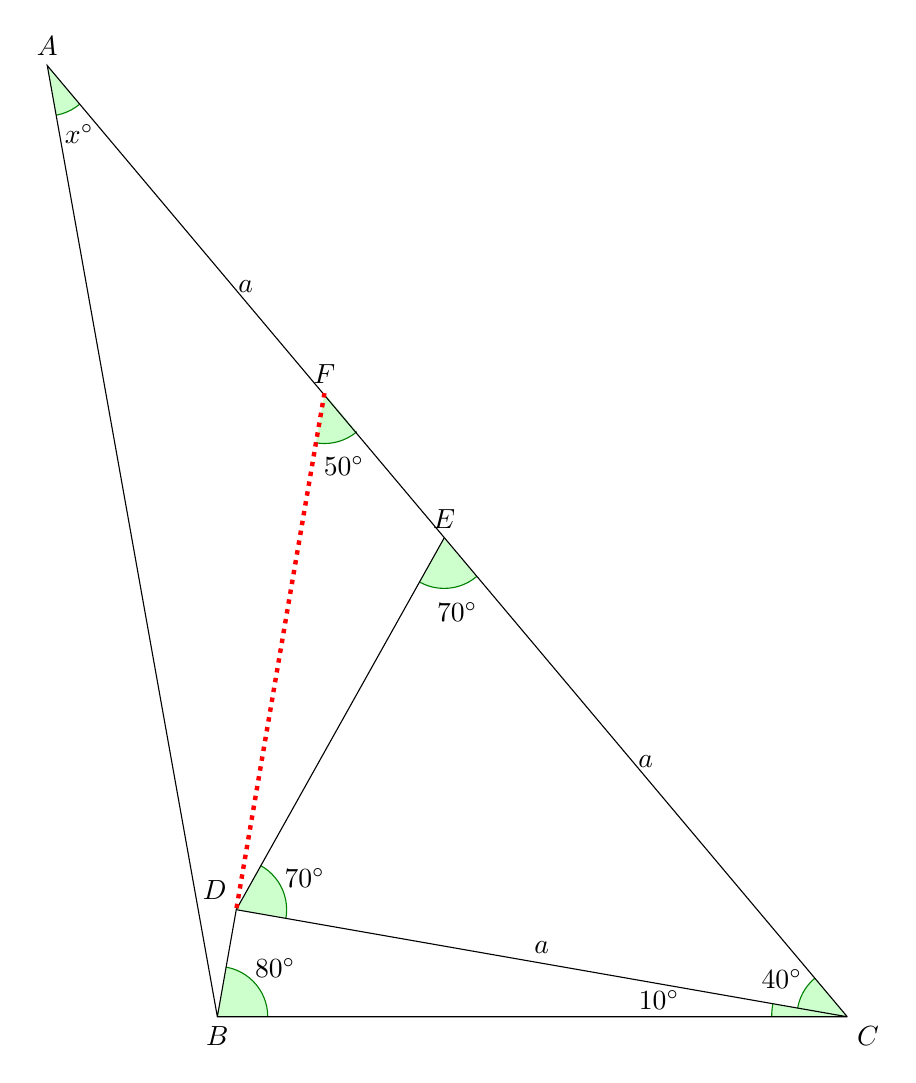
\begin{tikzpicture}[x=\figuresize,y=\figuresize]
	\coordinate [label=below:$B$] (B) at (0,0);
	\coordinate [label=below right:$C$] (C) at (1,0);
	\coordinate [label=above left:$D$] (D) at (0.03,0.17);
	\coordinate [label=above:$A$] (A) at (-0.27,1.51);
	\coordinate [label=above:$E$] (E) at (0.36,0.76);
	\coordinate [label=above:$F$] (F) at (0.17,0.99);
	\coordinate (AEmid) at ($(A)!0.5!(E)$);
	\coordinate (CEmid) at ($(C)!0.5!(E)$);
	\coordinate (CDmid) at ($(C)!0.5!(D)$);

	\node at (CDmid)[above] {$a$};
	\node at (AEmid)[above] {$a$};
	\node at (CEmid)[above] {$a$};
	
	\makeangle{D}{B}{C}{80}{0.08}{40}{0.12}
	\makeangle{B}{C}{D}{10}{0.12}{175}{0.30}
	\makeangle{A}{C}{D}{40}{0.08}{150}{0.12}
	\makeangle{B}{A}{C}{x}{0.08}{295}{0.12}
	\makeangle{D}{E}{C}{70}{0.08}{280}{0.12}
	\makeangle{C}{D}{E}{70}{0.08}{25}{0.12}
	\makeangle{B}{F}{C}{50}{0.08}{285}{0.12}

	\draw (B) -- (D) -- (C) -- (B) -- (A) -- (C);
	\draw (E) -- (D);
	\draw[red, dotted, ultra thick] (F) -- (D);
	\end{tikzpicture}
	\caption{$\angle \hat{DEC} = 50\degree; \overline{BF} = \overline{BC}$}
\end{figure}

\begin{figure}
	\centering
	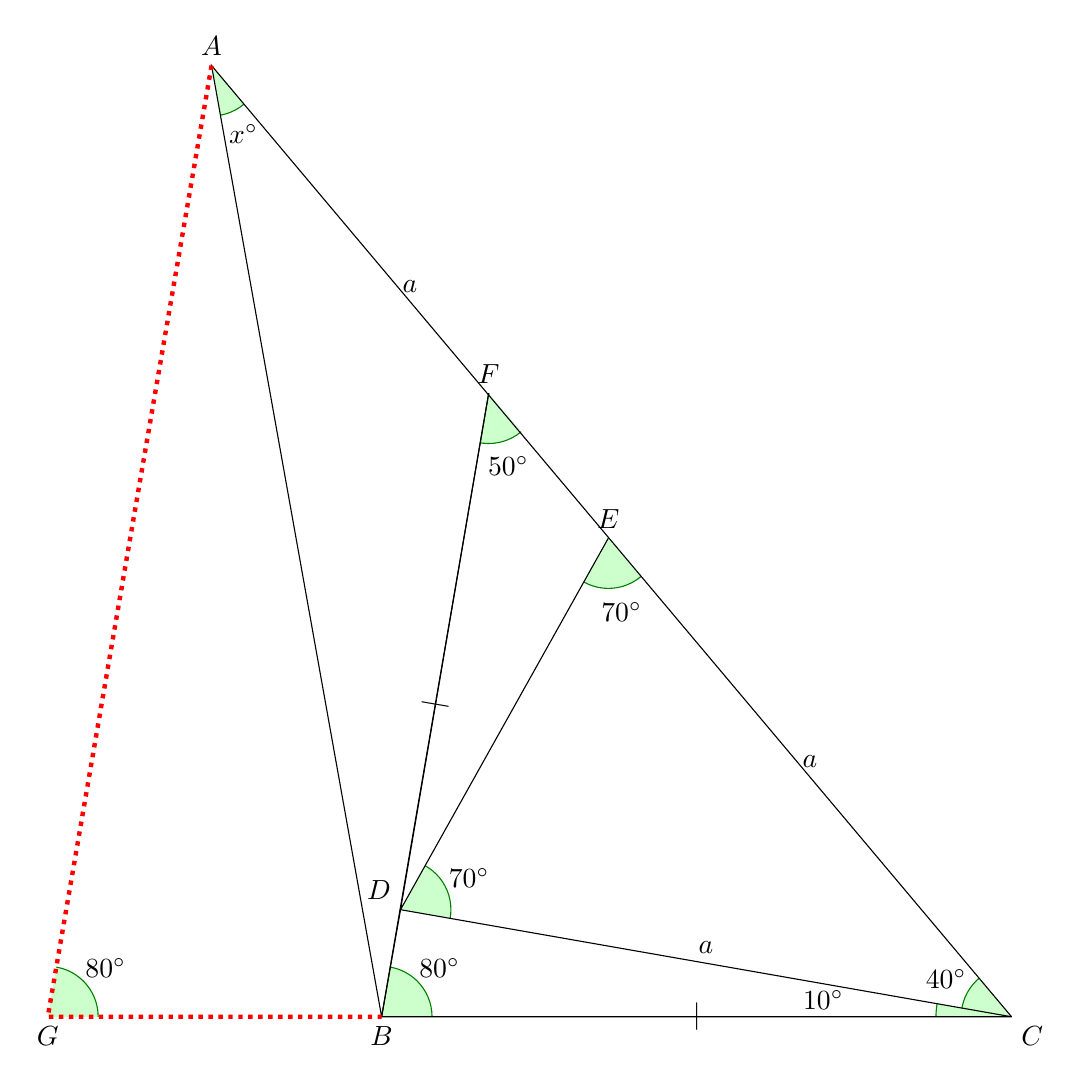
\begin{tikzpicture}[x=\figuresize,y=\figuresize]
	\coordinate [label=below:$B$] (B) at (0,0);
	\coordinate [label=below right:$C$] (C) at (1,0);
	\coordinate [label=above left:$D$] (D) at (0.03,0.17);
	\coordinate [label=above:$A$] (A) at (-0.27,1.51);
	\coordinate [label=above:$E$] (E) at (0.36,0.76);
	\coordinate [label=above:$F$] (F) at (0.17,0.99);
	\coordinate [label=below:$G$] (G) at (-0.53,0);
	\coordinate (AEmid) at ($(A)!0.5!(E)$);
	\coordinate (CEmid) at ($(C)!0.5!(E)$);
	\coordinate (CDmid) at ($(C)!0.5!(D)$);

	\node at (CDmid)[above] {$a$};
	\node at (AEmid)[above] {$a$};
	\node at (CEmid)[above] {$a$};
	
	\makeangle{D}{B}{C}{80}{0.08}{40}{0.12}
	\makeangle{B}{C}{D}{10}{0.12}{175}{0.30}
	\makeangle{A}{C}{D}{40}{0.08}{150}{0.12}
	\makeangle{B}{A}{C}{x}{0.08}{295}{0.12}
	\makeangle{D}{E}{C}{70}{0.08}{280}{0.12}
	\makeangle{C}{D}{E}{70}{0.08}{25}{0.12}
	\makeangle{B}{F}{C}{50}{0.08}{285}{0.12}
	\makeangle{A}{G}{B}{80}{0.08}{40}{0.12}

	\draw (B) -- (D) -- (C) -- (B) -- (A) -- (C);
	\draw (E) -- (D) -- (F);
	\draw (B) -- node[sloped] {$|$} (C);
	\draw (B) -- node[sloped] {$|$} (F);
	\draw[red, dotted, ultra thick] (A) -- (G) -- (B);
	\end{tikzpicture}
	\caption{$\overline{GA}//\overline{BF}; \angle \hat{BGA} = \angle \hat{FBC} = 80\degree; \overline{AG} = \overline{CG}; \triangle FBC \approx \triangle AGC$}
\end{figure}

\begin{figure}
	\centering
	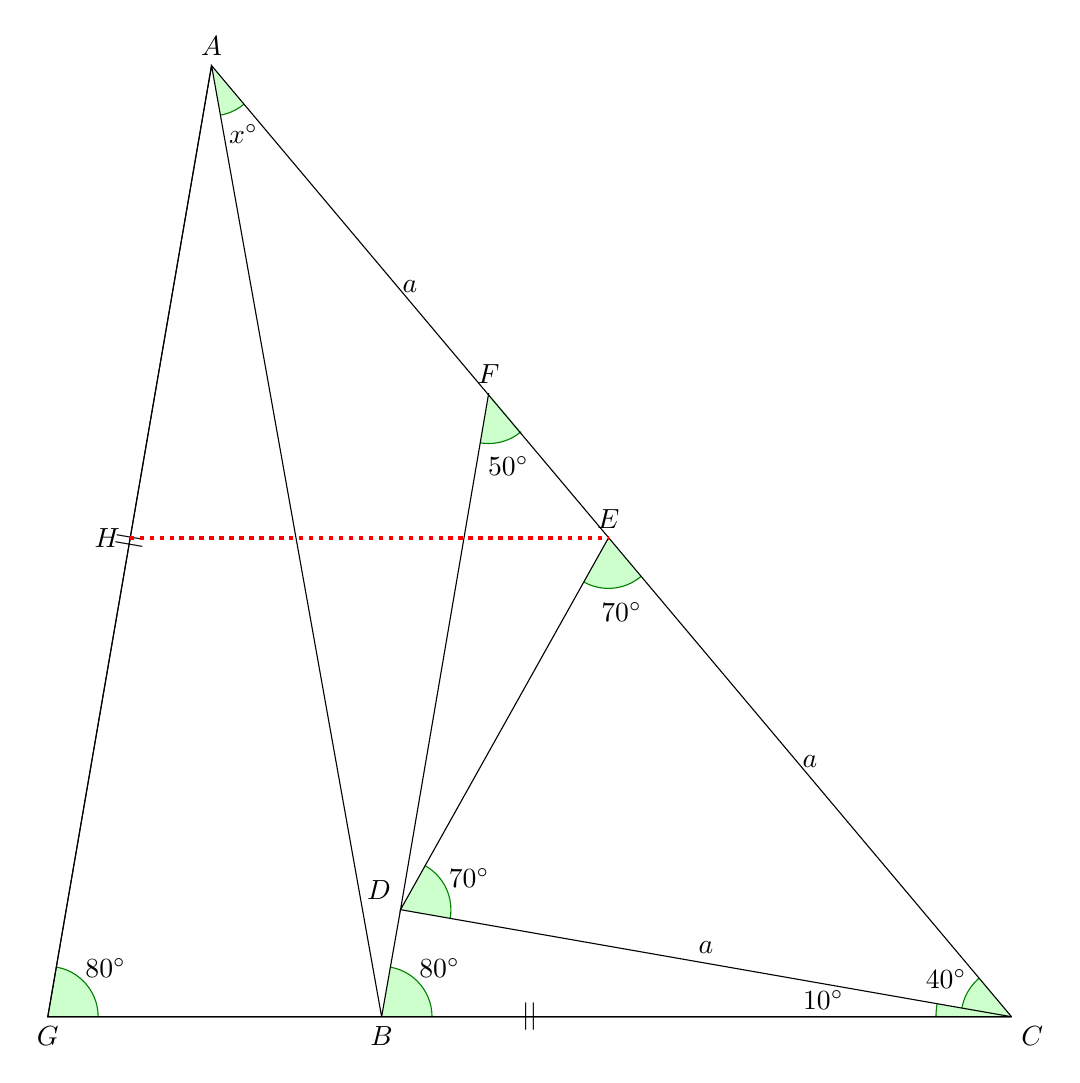
\begin{tikzpicture}[x=\figuresize,y=\figuresize]
	\coordinate [label=below:$B$] (B) at (0,0);
	\coordinate [label=below right:$C$] (C) at (1,0);
	\coordinate [label=above left:$D$] (D) at (0.03,0.17);
	\coordinate [label=above:$A$] (A) at (-0.27,1.51);
	\coordinate [label=above:$E$] (E) at (0.36,0.76);
	\coordinate [label=above:$F$] (F) at (0.17,0.99);
	\coordinate [label=below:$G$] (G) at (-0.53,0);
	\coordinate [label=left:$H$] (H) at (-0.4,0.76);
	\coordinate (AEmid) at ($(A)!0.5!(E)$);
	\coordinate (CEmid) at ($(C)!0.5!(E)$);
	\coordinate (CDmid) at ($(C)!0.5!(D)$);

	\node at (CDmid)[above] {$a$};
	\node at (AEmid)[above] {$a$};
	\node at (CEmid)[above] {$a$};
	
	\makeangle{D}{B}{C}{80}{0.08}{40}{0.12}
	\makeangle{B}{C}{D}{10}{0.12}{175}{0.30}
	\makeangle{A}{C}{D}{40}{0.08}{150}{0.12}
	\makeangle{B}{A}{C}{x}{0.08}{295}{0.12}
	\makeangle{D}{E}{C}{70}{0.08}{280}{0.12}
	\makeangle{C}{D}{E}{70}{0.08}{25}{0.12}
	\makeangle{B}{F}{C}{50}{0.08}{285}{0.12}
	\makeangle{A}{G}{B}{80}{0.08}{40}{0.12}

	\draw (A) -- (G) -- (B) -- (D) -- (C) -- (B) -- (A) -- (C);
	\draw (E) -- (D) -- (F);
	\draw (A) -- node[sloped] {$||$} (G) -- node[sloped] {$||$} (C);
	\draw[red, dotted, ultra thick] (H) -- (E);
	\end{tikzpicture}
	\caption{$\overline{HE}//\overline{GC}; \angle \hat{AHE} = 80\degree; \hat{HAE} = \hat{HEA} = 50\degree; \overline{GH} = \overline{HE} = \overline{HA}$}
\end{figure}

\begin{figure}
	\centering
	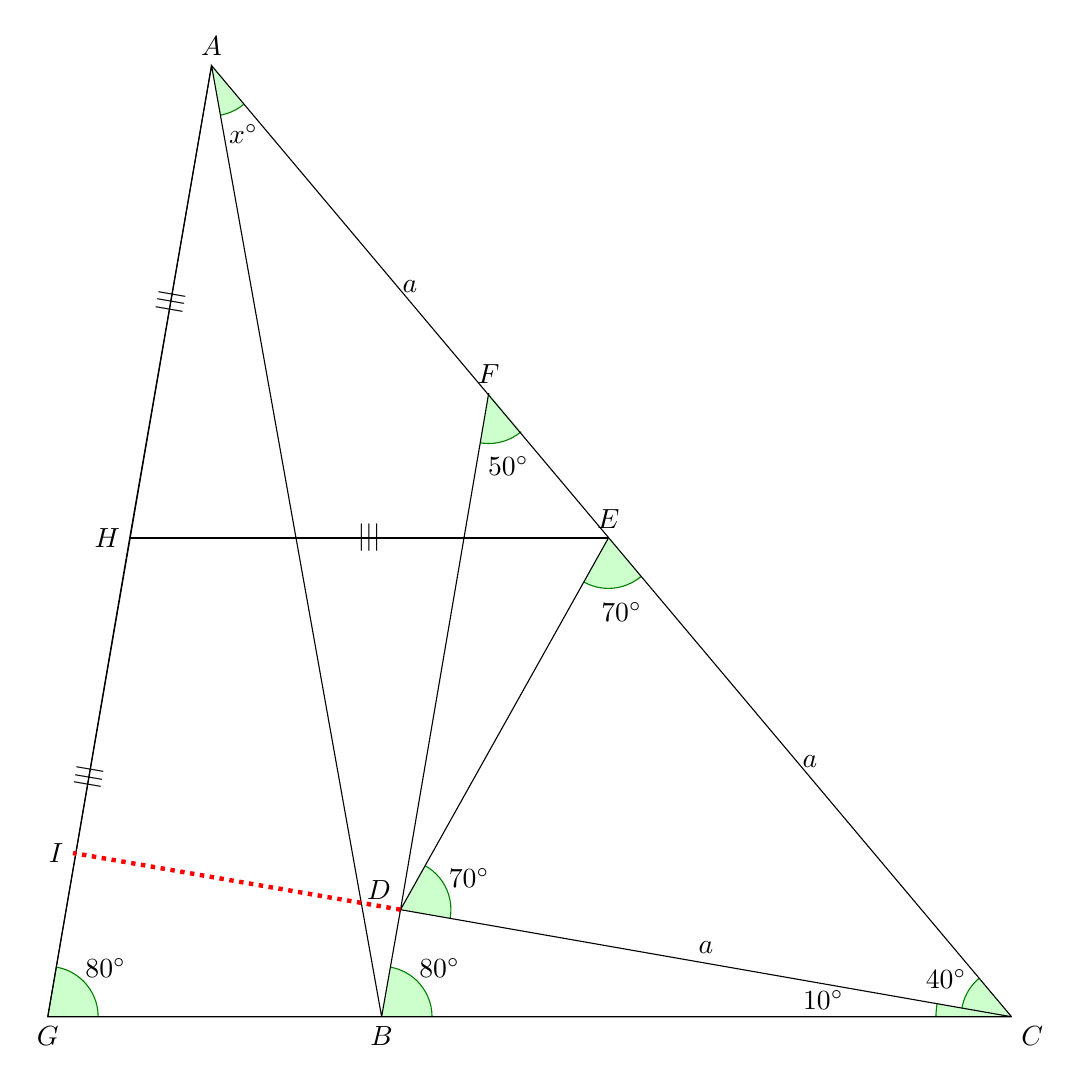
\begin{tikzpicture}[x=\figuresize,y=\figuresize]
	\coordinate [label=below:$B$] (B) at (0,0);
	\coordinate [label=below right:$C$] (C) at (1,0);
	\coordinate [label=above left:$D$] (D) at (0.03,0.17);
	\coordinate [label=above:$A$] (A) at (-0.27,1.51);
	\coordinate [label=above:$E$] (E) at (0.36,0.76);
	\coordinate [label=above:$F$] (F) at (0.17,0.99);
	\coordinate [label=below:$G$] (G) at (-0.53,0);
	\coordinate [label=left:$H$] (H) at (-0.4,0.76);
	\coordinate [label=left:$I$] (I) at (-0.49,0.26);
	\coordinate (AEmid) at ($(A)!0.5!(E)$);
	\coordinate (CEmid) at ($(C)!0.5!(E)$);
	\coordinate (CDmid) at ($(C)!0.5!(D)$);

	\node at (CDmid)[above] {$a$};
	\node at (AEmid)[above] {$a$};
	\node at (CEmid)[above] {$a$};
	
	\makeangle{D}{B}{C}{80}{0.08}{40}{0.12}
	\makeangle{B}{C}{D}{10}{0.12}{175}{0.30}
	\makeangle{A}{C}{D}{40}{0.08}{150}{0.12}
	\makeangle{B}{A}{C}{x}{0.08}{295}{0.12}
	\makeangle{D}{E}{C}{70}{0.08}{280}{0.12}
	\makeangle{C}{D}{E}{70}{0.08}{25}{0.12}
	\makeangle{B}{F}{C}{50}{0.08}{285}{0.12}
	\makeangle{A}{G}{B}{80}{0.08}{40}{0.12}

	\draw (A) -- (G) -- (B) -- (D) -- (C) -- (B) -- (A) -- (C);
	\draw (E) -- (D) -- (F);
	\draw (A) -- node[sloped] {$|||$} (H) -- node[sloped] {$|||$} (G);
	\draw (E) -- node[sloped] {$|||$} (H);
	\draw[red, dotted, ultra thick] (D) -- (I);
	\end{tikzpicture}
	\caption{$\angle \hat{GIC} = \angle \hat{BDC} = 90\degree$}
\end{figure}

\begin{figure}
	\centering
	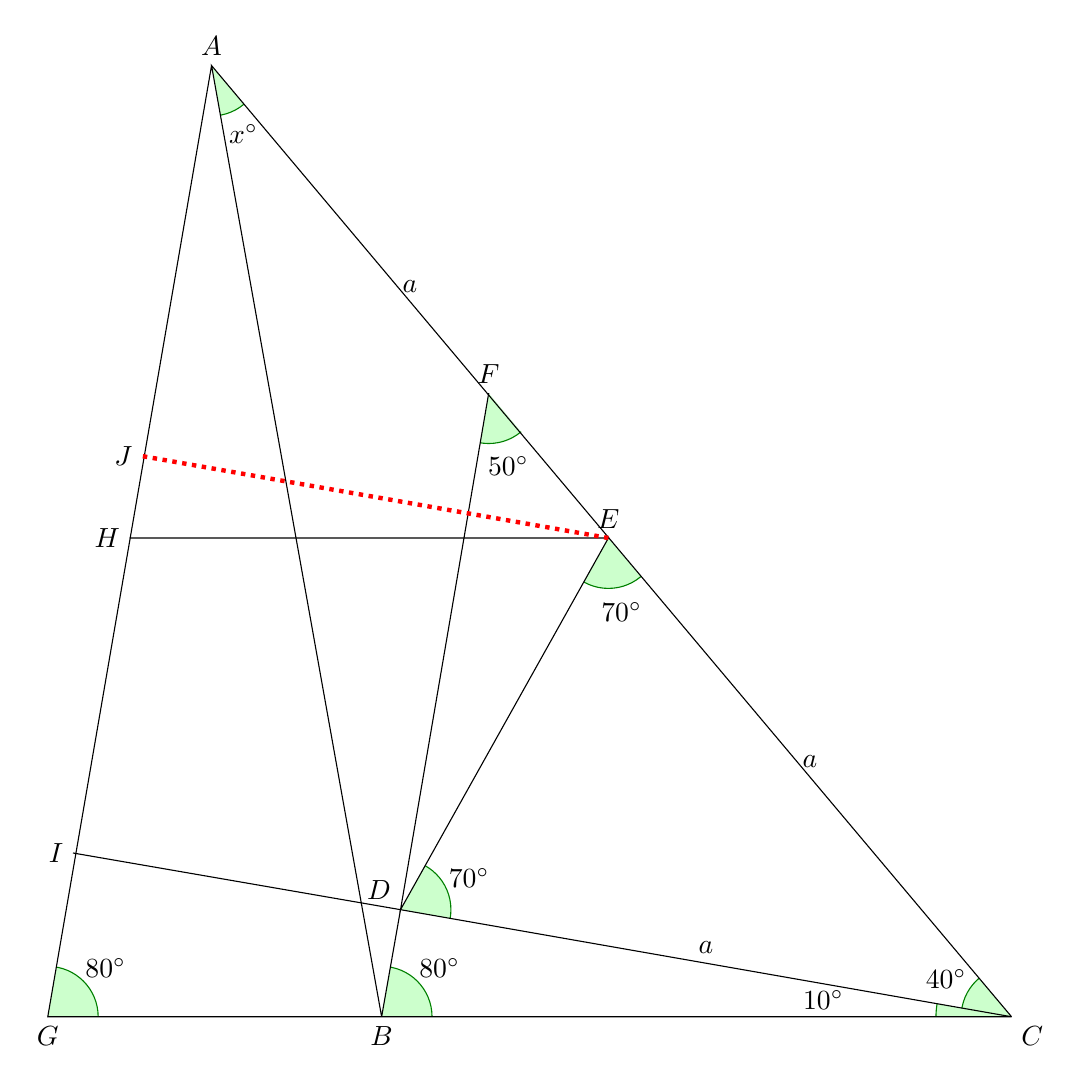
\begin{tikzpicture}[x=\figuresize,y=\figuresize]
	\coordinate [label=below:$B$] (B) at (0,0);
	\coordinate [label=below right:$C$] (C) at (1,0);
	\coordinate [label=above left:$D$] (D) at (0.03,0.17);
	\coordinate [label=above:$A$] (A) at (-0.27,1.51);
	\coordinate [label=above:$E$] (E) at (0.36,0.76);
	\coordinate [label=above:$F$] (F) at (0.17,0.99);
	\coordinate [label=below:$G$] (G) at (-0.53,0);
	\coordinate [label=left:$H$] (H) at (-0.4,0.76);
	\coordinate [label=left:$I$] (I) at (-0.49,0.26);
	\coordinate [label=left:$J$] (J) at (-0.38,0.89);
	\coordinate (AEmid) at ($(A)!0.5!(E)$);
	\coordinate (CEmid) at ($(C)!0.5!(E)$);
	\coordinate (CDmid) at ($(C)!0.5!(D)$);

	\node at (CDmid)[above] {$a$};
	\node at (AEmid)[above] {$a$};
	\node at (CEmid)[above] {$a$};
	
	\makeangle{D}{B}{C}{80}{0.08}{40}{0.12}
	\makeangle{B}{C}{D}{10}{0.12}{175}{0.30}
	\makeangle{A}{C}{D}{40}{0.08}{150}{0.12}
	\makeangle{B}{A}{C}{x}{0.08}{295}{0.12}
	\makeangle{D}{E}{C}{70}{0.08}{280}{0.12}
	\makeangle{C}{D}{E}{70}{0.08}{25}{0.12}
	\makeangle{B}{F}{C}{50}{0.08}{285}{0.12}
	\makeangle{A}{G}{B}{80}{0.08}{40}{0.12}

	\draw (A) -- (G) -- (B) -- (D) -- (C) -- (B) -- (A) -- (C);
	\draw (H) -- (E) -- (D) -- (F);
	\draw (D) -- (I);
	\draw[red, dotted, ultra thick] (E) -- (J);
	\end{tikzpicture}
	\caption{$\triangle HJE \approx \triangle BDC$}
\end{figure}

\begin{figure}
	\centering
	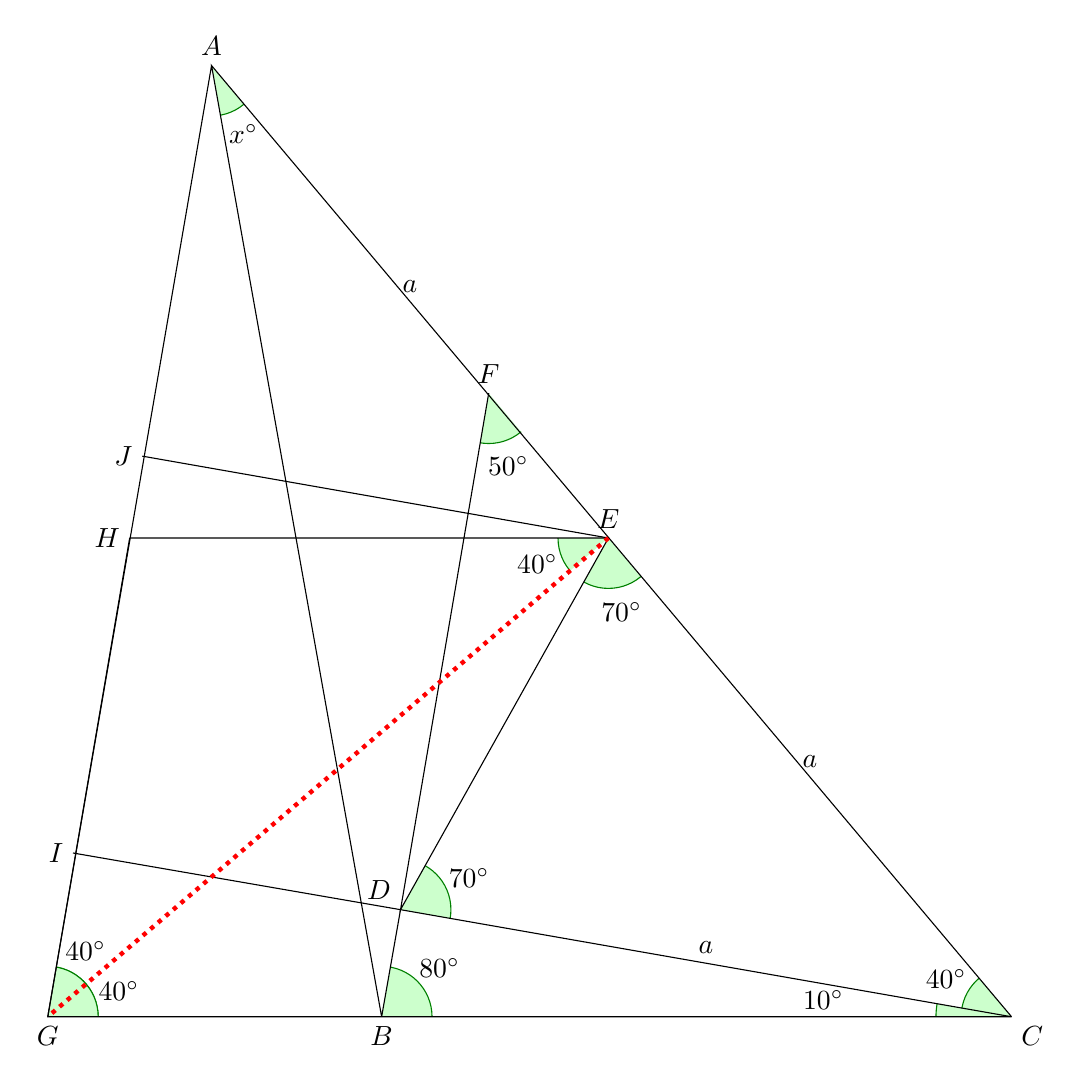
\begin{tikzpicture}[x=\figuresize,y=\figuresize]
	\coordinate [label=below:$B$] (B) at (0,0);
	\coordinate [label=below right:$C$] (C) at (1,0);
	\coordinate [label=above left:$D$] (D) at (0.03,0.17);
	\coordinate [label=above:$A$] (A) at (-0.27,1.51);
	\coordinate [label=above:$E$] (E) at (0.36,0.76);
	\coordinate [label=above:$F$] (F) at (0.17,0.99);
	\coordinate [label=below:$G$] (G) at (-0.53,0);
	\coordinate [label=left:$H$] (H) at (-0.4,0.76);
	\coordinate [label=left:$I$] (I) at (-0.49,0.26);
	\coordinate [label=left:$J$] (J) at (-0.38,0.89);
	\coordinate (AEmid) at ($(A)!0.5!(E)$);
	\coordinate (CEmid) at ($(C)!0.5!(E)$);
	\coordinate (CDmid) at ($(C)!0.5!(D)$);

	\node at (CDmid)[above] {$a$};
	\node at (AEmid)[above] {$a$};
	\node at (CEmid)[above] {$a$};
	
	\makeangle{D}{B}{C}{80}{0.08}{40}{0.12}
	\makeangle{B}{C}{D}{10}{0.12}{175}{0.30}
	\makeangle{A}{C}{D}{40}{0.08}{150}{0.12}
	\makeangle{B}{A}{C}{x}{0.08}{295}{0.12}
	\makeangle{D}{E}{C}{70}{0.08}{280}{0.12}
	\makeangle{C}{D}{E}{70}{0.08}{25}{0.12}
	\makeangle{B}{F}{C}{50}{0.08}{285}{0.12}
	\makeangle{A}{G}{B}{40}{0.08}{20}{0.12}
	\makeangle{A}{G}{B}{40}{0.08}{60}{0.12}
	\makeangle{H}{E}{G}{40}{0.08}{200}{0.12}

	\draw (A) -- (G) -- (B) -- (D) -- (C) -- (B) -- (A) -- (C);
	\draw (H) -- (E) -- (D) -- (F);
	\draw (H) -- (G);
	\draw (D) -- (I);
	\draw (E) -- (J);
	\draw[red, dotted, ultra thick] (E) -- (G);
	\end{tikzpicture}
	\caption{$\overline{GH} = \overline{HE} \therefore \angle \hat{HGE} = \angle \hat{HEG} = 40\degree$}
\end{figure}

\begin{figure}
	\centering
	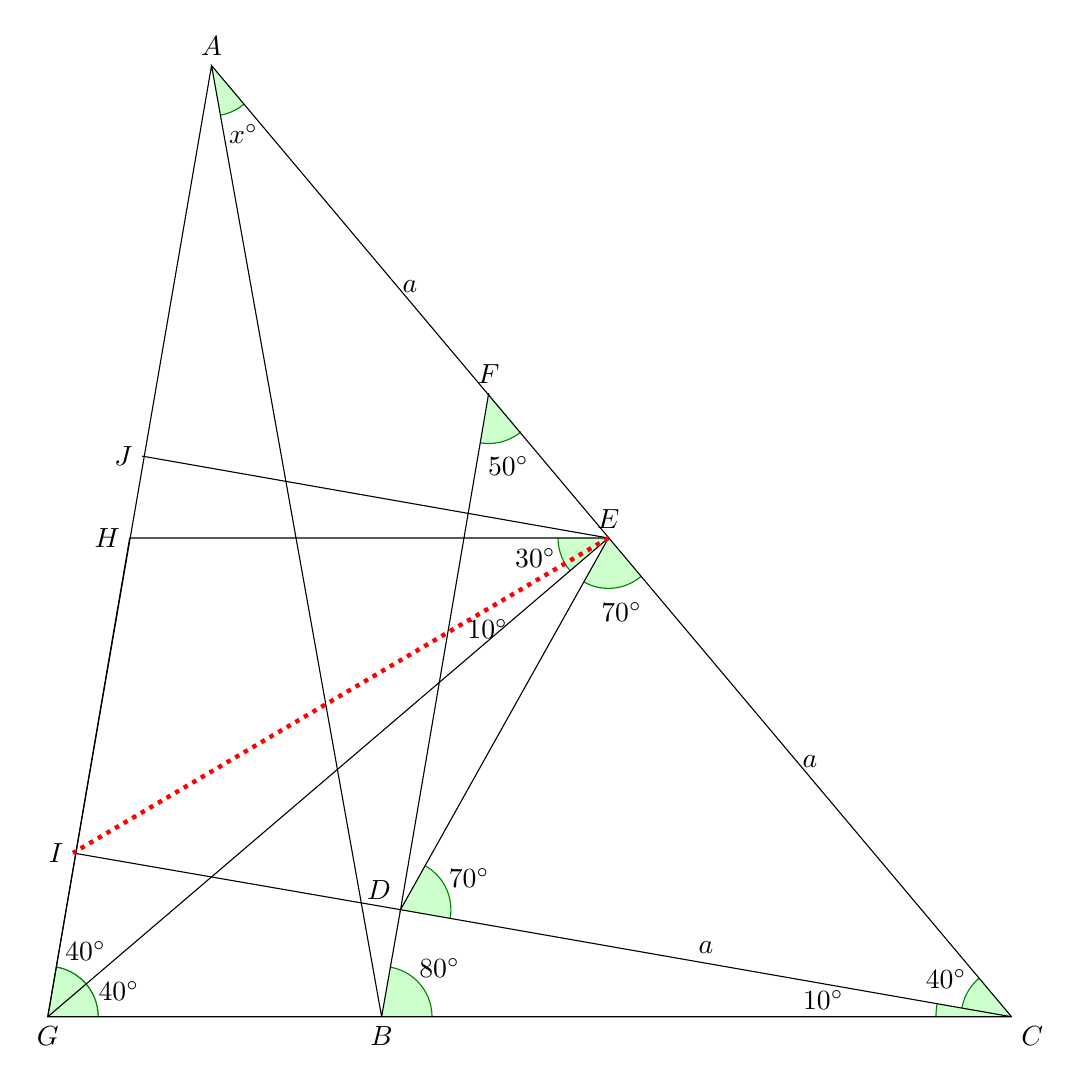
\begin{tikzpicture}[x=\figuresize,y=\figuresize]
	\coordinate [label=below:$B$] (B) at (0,0);
	\coordinate [label=below right:$C$] (C) at (1,0);
	\coordinate [label=above left:$D$] (D) at (0.03,0.17);
	\coordinate [label=above:$A$] (A) at (-0.27,1.51);
	\coordinate [label=above:$E$] (E) at (0.36,0.76);
	\coordinate [label=above:$F$] (F) at (0.17,0.99);
	\coordinate [label=below:$G$] (G) at (-0.53,0);
	\coordinate [label=left:$H$] (H) at (-0.4,0.76);
	\coordinate [label=left:$I$] (I) at (-0.49,0.26);
	\coordinate [label=left:$J$] (J) at (-0.38,0.89);
	\coordinate (AEmid) at ($(A)!0.5!(E)$);
	\coordinate (CEmid) at ($(C)!0.5!(E)$);
	\coordinate (CDmid) at ($(C)!0.5!(D)$);

	\node at (CDmid)[above] {$a$};
	\node at (AEmid)[above] {$a$};
	\node at (CEmid)[above] {$a$};
	
	\makeangle{D}{B}{C}{80}{0.08}{40}{0.12}
	\makeangle{B}{C}{D}{10}{0.12}{175}{0.30}
	\makeangle{A}{C}{D}{40}{0.08}{150}{0.12}
	\makeangle{B}{A}{C}{x}{0.08}{295}{0.12}
	\makeangle{D}{E}{C}{70}{0.08}{280}{0.12}
	\makeangle{C}{D}{E}{70}{0.08}{25}{0.12}
	\makeangle{B}{F}{C}{50}{0.08}{285}{0.12}
	\makeangle{A}{G}{B}{40}{0.08}{20}{0.12}
	\makeangle{A}{G}{B}{40}{0.08}{60}{0.12}
	\makeangle{H}{E}{I}{30}{0.08}{195}{0.12}
	\makeangle{I}{E}{G}{10}{0.08}{217}{0.24}

	\draw (A) -- (G) -- (B) -- (D) -- (C) -- (B) -- (A) -- (C);
	\draw (H) -- (E) -- (D) -- (F);
	\draw (H) -- (G);
	\draw (D) -- (I);
	\draw (G) -- (E) -- (J);
	\draw[red, dotted, ultra thick] (E) -- (I);
	\end{tikzpicture}
	\caption{$\overline{AE} = \overline{IE} = \overline{EC}$}
\end{figure}

\begin{figure}
	\centering
	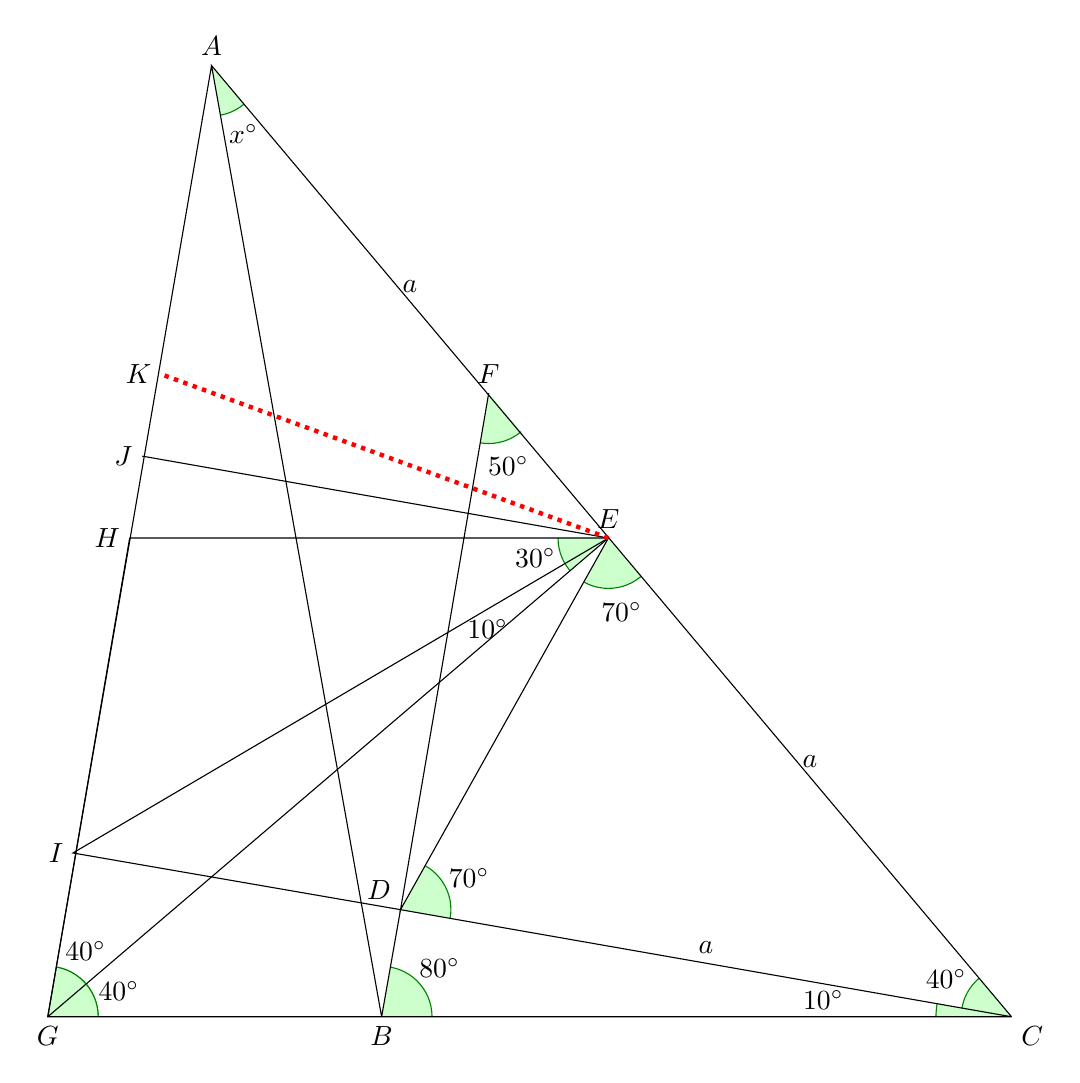
\begin{tikzpicture}[x=\figuresize,y=\figuresize]
	\coordinate [label=below:$B$] (B) at (0,0);
	\coordinate [label=below right:$C$] (C) at (1,0);
	\coordinate [label=above left:$D$] (D) at (0.03,0.17);
	\coordinate [label=above:$A$] (A) at (-0.27,1.51);
	\coordinate [label=above:$E$] (E) at (0.36,0.76);
	\coordinate [label=above:$F$] (F) at (0.17,0.99);
	\coordinate [label=below:$G$] (G) at (-0.53,0);
	\coordinate [label=left:$H$] (H) at (-0.4,0.76);
	\coordinate [label=left:$I$] (I) at (-0.49,0.26);
	\coordinate [label=left:$J$] (J) at (-0.38,0.89);
	\coordinate [label=left:$K$] (K) at (-0.35,1.02);
	\coordinate (AEmid) at ($(A)!0.5!(E)$);
	\coordinate (CEmid) at ($(C)!0.5!(E)$);
	\coordinate (CDmid) at ($(C)!0.5!(D)$);

	\node at (CDmid)[above] {$a$};
	\node at (AEmid)[above] {$a$};
	\node at (CEmid)[above] {$a$};
	
	\makeangle{D}{B}{C}{80}{0.08}{40}{0.12}
	\makeangle{B}{C}{D}{10}{0.12}{175}{0.30}
	\makeangle{A}{C}{D}{40}{0.08}{150}{0.12}
	\makeangle{B}{A}{C}{x}{0.08}{295}{0.12}
	\makeangle{D}{E}{C}{70}{0.08}{280}{0.12}
	\makeangle{C}{D}{E}{70}{0.08}{25}{0.12}
	\makeangle{B}{F}{C}{50}{0.08}{285}{0.12}
	\makeangle{A}{G}{B}{40}{0.08}{20}{0.12}
	\makeangle{A}{G}{B}{40}{0.08}{60}{0.12}
	\makeangle{H}{E}{I}{30}{0.08}{195}{0.12}
	\makeangle{I}{E}{G}{10}{0.08}{217}{0.24}

	\draw (A) -- (G) -- (B) -- (D) -- (C) -- (B) -- (A) -- (C);
	\draw (H) -- (E) -- (D) -- (F);
	\draw (H) -- (G);
	\draw (D) -- (I) -- (E);
	\draw (G) -- (E) -- (J);
	\draw[red, dotted, ultra thick] (E) -- (K);
	\end{tikzpicture}
	\caption{$\triangle HJE \equiv \triangle KJE; \triangle KIE \approx \triangle BCF$}
\end{figure}

\begin{figure}
	\centering
	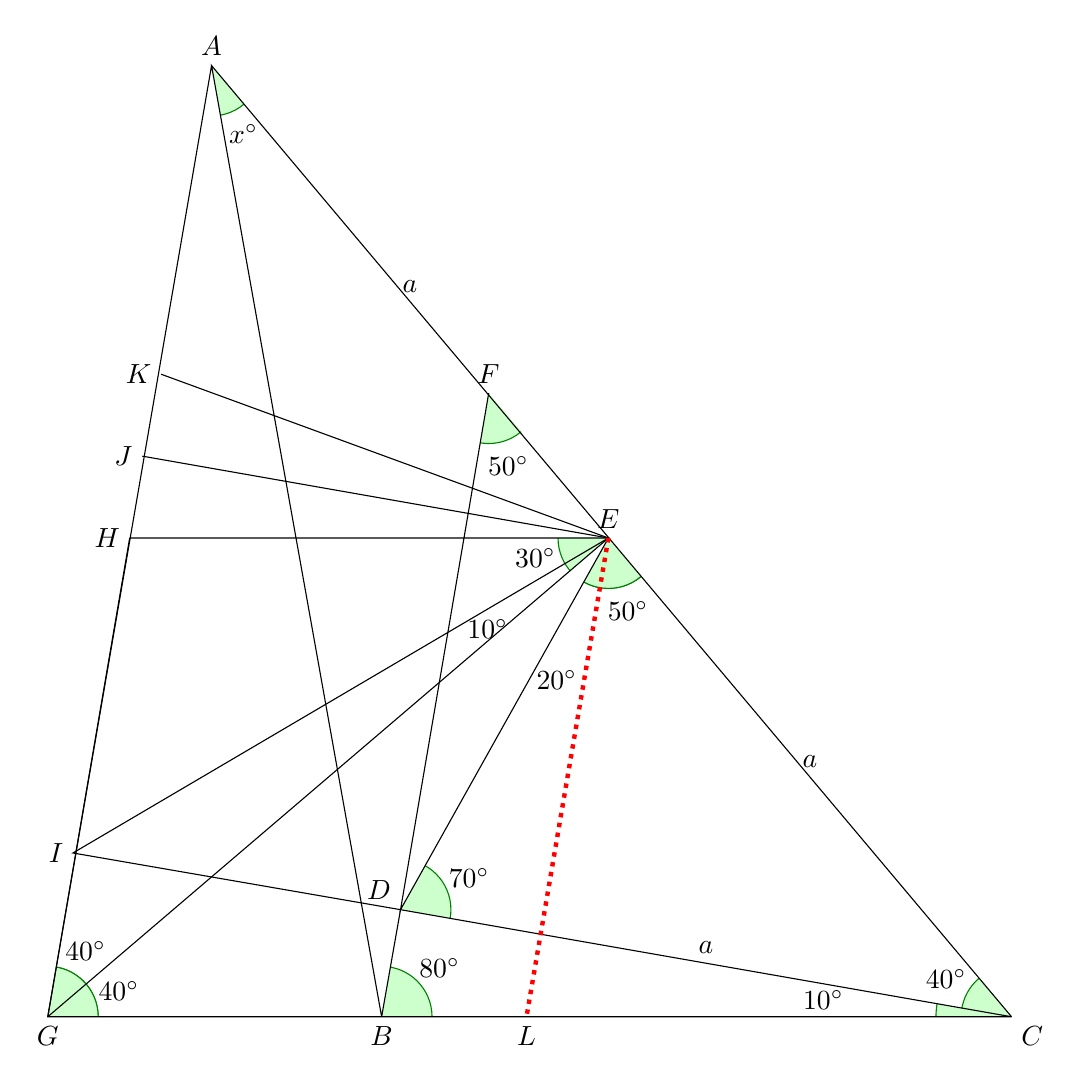
\begin{tikzpicture}[x=\figuresize,y=\figuresize]
	\coordinate [label=below:$B$] (B) at (0,0);
	\coordinate [label=below right:$C$] (C) at (1,0);
	\coordinate [label=above left:$D$] (D) at (0.03,0.17);
	\coordinate [label=above:$A$] (A) at (-0.27,1.51);
	\coordinate [label=above:$E$] (E) at (0.36,0.76);
	\coordinate [label=above:$F$] (F) at (0.17,0.99);
	\coordinate [label=below:$G$] (G) at (-0.53,0);
	\coordinate [label=left:$H$] (H) at (-0.4,0.76);
	\coordinate [label=left:$I$] (I) at (-0.49,0.26);
	\coordinate [label=left:$J$] (J) at (-0.38,0.89);
	\coordinate [label=left:$K$] (K) at (-0.35,1.02);
	\coordinate [label=below:$L$] (L) at (0.23,0);
	\coordinate (AEmid) at ($(A)!0.5!(E)$);
	\coordinate (CEmid) at ($(C)!0.5!(E)$);
	\coordinate (CDmid) at ($(C)!0.5!(D)$);

	\node at (CDmid)[above] {$a$};
	\node at (AEmid)[above] {$a$};
	\node at (CEmid)[above] {$a$};
	
	\makeangle{D}{B}{C}{80}{0.08}{40}{0.12}
	\makeangle{B}{C}{D}{10}{0.12}{175}{0.30}
	\makeangle{A}{C}{D}{40}{0.08}{150}{0.12}
	\makeangle{B}{A}{C}{x}{0.08}{295}{0.12}
	\makeangle{D}{E}{C}{50}{0.08}{285}{0.12}
	\makeangle{D}{E}{C}{20}{0.08}{250}{0.24}
	\makeangle{C}{D}{E}{70}{0.08}{25}{0.12}
	\makeangle{B}{F}{C}{50}{0.08}{285}{0.12}
	\makeangle{A}{G}{B}{40}{0.08}{20}{0.12}
	\makeangle{A}{G}{B}{40}{0.08}{60}{0.12}
	\makeangle{H}{E}{I}{30}{0.08}{195}{0.12}
	\makeangle{I}{E}{G}{10}{0.08}{217}{0.24}

	\draw (A) -- (G) -- (B) -- (D) -- (C) -- (B) -- (A) -- (C);
	\draw (H) -- (E) -- (D) -- (F);
	\draw (H) -- (G);
	\draw (D) -- (I) -- (E) -- (K);
	\draw (G) -- (E) -- (J);
	\draw[red, dotted, ultra thick] (E) -- (L);
	\end{tikzpicture}
	\caption{$\triangle HJE \equiv \triangle KJE; \triangle KIE \approx \triangle BCF$}
\end{figure}

\begin{figure}
	\centering
	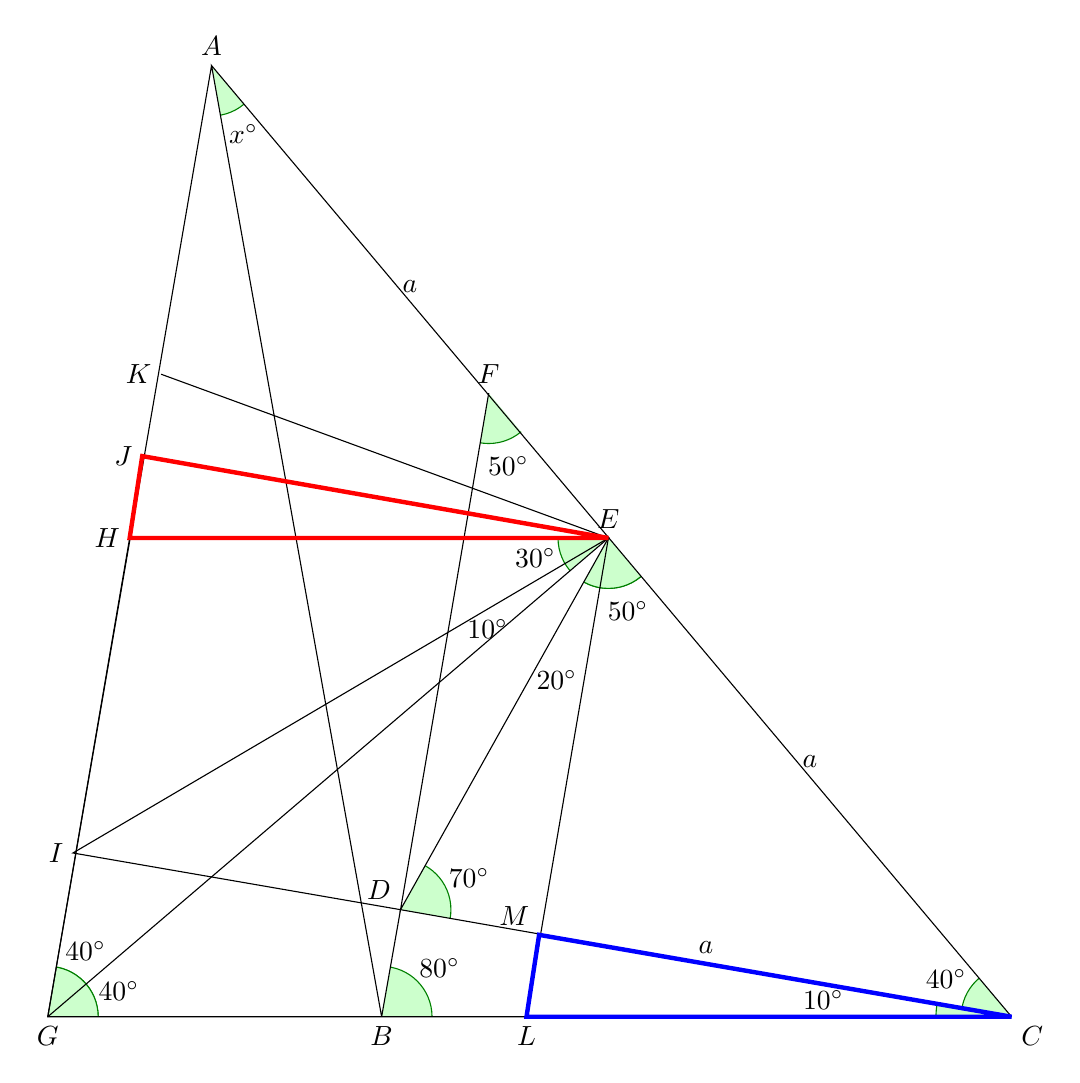
\begin{tikzpicture}[x=\figuresize,y=\figuresize]
	\coordinate [label=below:$B$] (B) at (0,0);
	\coordinate [label=below right:$C$] (C) at (1,0);
	\coordinate [label=above left:$D$] (D) at (0.03,0.17);
	\coordinate [label=above:$A$] (A) at (-0.27,1.51);
	\coordinate [label=above:$E$] (E) at (0.36,0.76);
	\coordinate [label=above:$F$] (F) at (0.17,0.99);
	\coordinate [label=below:$G$] (G) at (-0.53,0);
	\coordinate [label=left:$H$] (H) at (-0.4,0.76);
	\coordinate [label=left:$I$] (I) at (-0.49,0.26);
	\coordinate [label=left:$J$] (J) at (-0.38,0.89);
	\coordinate [label=left:$K$] (K) at (-0.35,1.02);
	\coordinate [label=below:$L$] (L) at (0.23,0);
	\coordinate [label=above left:$M$] (M) at (0.25,0.13);
	\coordinate (AEmid) at ($(A)!0.5!(E)$);
	\coordinate (CEmid) at ($(C)!0.5!(E)$);
	\coordinate (CDmid) at ($(C)!0.5!(D)$);

	\node at (CDmid)[above] {$a$};
	\node at (AEmid)[above] {$a$};
	\node at (CEmid)[above] {$a$};
	
	\makeangle{D}{B}{C}{80}{0.08}{40}{0.12}
	\makeangle{B}{C}{D}{10}{0.12}{175}{0.30}
	\makeangle{A}{C}{D}{40}{0.08}{150}{0.12}
	\makeangle{B}{A}{C}{x}{0.08}{295}{0.12}
	\makeangle{D}{E}{C}{50}{0.08}{285}{0.12}
	\makeangle{D}{E}{C}{20}{0.08}{250}{0.24}
	\makeangle{C}{D}{E}{70}{0.08}{25}{0.12}
	\makeangle{B}{F}{C}{50}{0.08}{285}{0.12}
	\makeangle{A}{G}{B}{40}{0.08}{20}{0.12}
	\makeangle{A}{G}{B}{40}{0.08}{60}{0.12}
	\makeangle{H}{E}{I}{30}{0.08}{195}{0.12}
	\makeangle{I}{E}{G}{10}{0.08}{217}{0.24}

	\draw (A) -- (G) -- (B) -- (D) -- (C) -- (B) -- (A) -- (C);
	\draw (H) -- (E) -- (D) -- (F);
	\draw (H) -- (G);
	\draw (D) -- (I) -- (E) -- (K);
	\draw (G) -- (E) -- (J);
	\draw (E) -- (L);
	\draw[blue, ultra thick] (M) -- (L) -- (C) -- cycle;
	\draw[red, ultra thick] (J) -- (H) -- (E) -- cycle;
	\end{tikzpicture}
	\caption{$\overline{JH} = \overline{ML} = \overline{KJ} = \frac{\overline{IG}}{2} \therefore \overline{KH} = \overline{ML}$}
\end{figure}

\begin{figure}
	\centering
	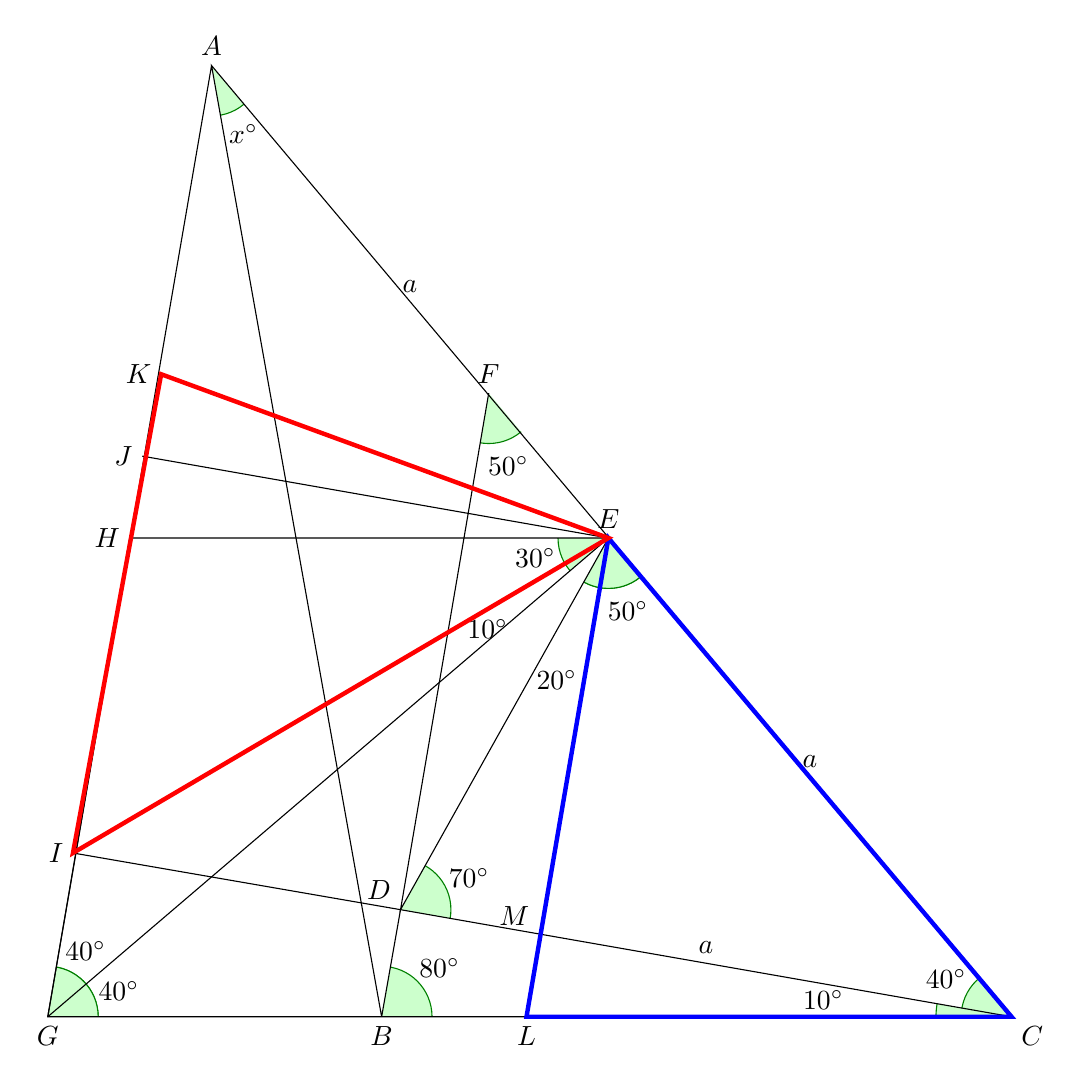
\begin{tikzpicture}[x=\figuresize,y=\figuresize]
	\coordinate [label=below:$B$] (B) at (0,0);
	\coordinate [label=below right:$C$] (C) at (1,0);
	\coordinate [label=above left:$D$] (D) at (0.03,0.17); \coordinate [label=above:$A$] (A) at (-0.27,1.51);
	\coordinate [label=above:$E$] (E) at (0.36,0.76);
	\coordinate [label=above:$F$] (F) at (0.17,0.99);
	\coordinate [label=below:$G$] (G) at (-0.53,0);
	\coordinate [label=left:$H$] (H) at (-0.4,0.76);
	\coordinate [label=left:$I$] (I) at (-0.49,0.26);
	\coordinate [label=left:$J$] (J) at (-0.38,0.89);
	\coordinate [label=left:$K$] (K) at (-0.35,1.02);
	\coordinate [label=below:$L$] (L) at (0.23,0);
	\coordinate [label=above left:$M$] (M) at (0.25,0.13);
	\coordinate (AEmid) at ($(A)!0.5!(E)$);
	\coordinate (CEmid) at ($(C)!0.5!(E)$);
	\coordinate (CDmid) at ($(C)!0.5!(D)$);

	\node at (CDmid)[above] {$a$};
	\node at (AEmid)[above] {$a$};
	\node at (CEmid)[above] {$a$};
	
	\makeangle{D}{B}{C}{80}{0.08}{40}{0.12}
	\makeangle{B}{C}{D}{10}{0.12}{175}{0.30}
	\makeangle{A}{C}{D}{40}{0.08}{150}{0.12}
	\makeangle{B}{A}{C}{x}{0.08}{295}{0.12}
	\makeangle{D}{E}{C}{50}{0.08}{285}{0.12}
	\makeangle{D}{E}{C}{20}{0.08}{250}{0.24}
	\makeangle{C}{D}{E}{70}{0.08}{25}{0.12}
	\makeangle{B}{F}{C}{50}{0.08}{285}{0.12}
	\makeangle{A}{G}{B}{40}{0.08}{20}{0.12}
	\makeangle{A}{G}{B}{40}{0.08}{60}{0.12}
	\makeangle{H}{E}{I}{30}{0.08}{195}{0.12}
	\makeangle{I}{E}{G}{10}{0.08}{217}{0.24}

	\draw (A) -- (G) -- (B) -- (D) -- (C) -- (B) -- (A) -- (C);
	\draw (H) -- (E) -- (D) -- (F);
	\draw (H) -- (G);
	\draw (D) -- (I) -- (E) -- (K);
	\draw (G) -- (E) -- (J);
	\draw (E) -- (L);
	\draw[blue, ultra thick] (L) -- (E) -- (C) -- cycle;
	\draw[red, ultra thick] (K) -- (I) -- (E) -- cycle;
	\end{tikzpicture}
	\caption{$\overline{AG}//\overline{EL} \therefore \overline{AG} = 2\overline{EL}; \overline{KI} = \overline{LC}, \overline{KE} = \overline{LE}, \angle \hat{KIE} = \angle \hat{LCE} = 50\degree \therefore \triangle KIE \equiv \triangle LCE$}
\end{figure}

\begin{figure}
	\centering
	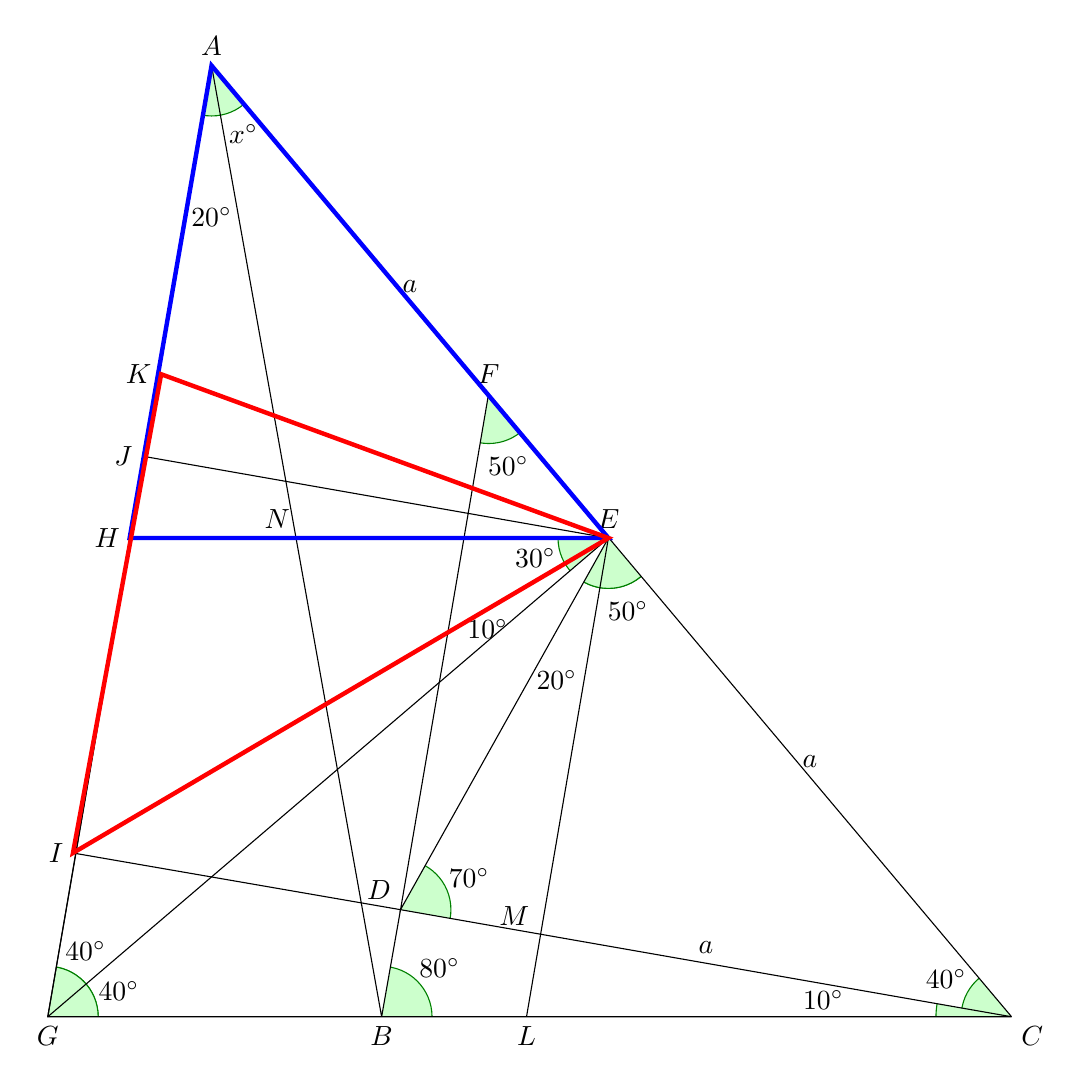
\begin{tikzpicture}[x=\figuresize,y=\figuresize]
	\coordinate [label=below:$B$] (B) at (0,0);
	\coordinate [label=below right:$C$] (C) at (1,0);
	\coordinate [label=above left:$D$] (D) at (0.03,0.17); \coordinate [label=above:$A$] (A) at (-0.27,1.51);
	\coordinate [label=above:$E$] (E) at (0.36,0.76);
	\coordinate [label=above:$F$] (F) at (0.17,0.99);
	\coordinate [label=below:$G$] (G) at (-0.53,0);
	\coordinate [label=left:$H$] (H) at (-0.4,0.76);
	\coordinate [label=left:$I$] (I) at (-0.49,0.26);
	\coordinate [label=left:$J$] (J) at (-0.38,0.89);
	\coordinate [label=left:$K$] (K) at (-0.35,1.02);
	\coordinate [label=below:$L$] (L) at (0.23,0);
	\coordinate [label=above left:$M$] (M) at (0.25,0.13);
	\coordinate [label=above left:$N$] (N) at (-0.13,0.76);
	\coordinate (AEmid) at ($(A)!0.5!(E)$);
	\coordinate (CEmid) at ($(C)!0.5!(E)$);
	\coordinate (CDmid) at ($(C)!0.5!(D)$);

	\node at (CDmid)[above] {$a$};
	\node at (AEmid)[above] {$a$};
	\node at (CEmid)[above] {$a$};
	
	\makeangle{D}{B}{C}{80}{0.08}{40}{0.12}
	\makeangle{B}{C}{D}{10}{0.12}{175}{0.30}
	\makeangle{A}{C}{D}{40}{0.08}{150}{0.12}
	\makeangle{B}{A}{C}{x}{0.08}{295}{0.12}
	\makeangle{D}{E}{C}{50}{0.08}{285}{0.12}
	\makeangle{D}{E}{C}{20}{0.08}{250}{0.24}
	\makeangle{C}{D}{E}{70}{0.08}{25}{0.12}
	\makeangle{B}{F}{C}{50}{0.08}{285}{0.12}
	\makeangle{A}{G}{B}{40}{0.08}{20}{0.12}
	\makeangle{A}{G}{B}{40}{0.08}{60}{0.12}
	\makeangle{H}{E}{I}{30}{0.08}{195}{0.12}
	\makeangle{I}{E}{G}{10}{0.08}{217}{0.24}
	\makeangle{B}{A}{G}{20}{0.08}{270}{0.24}

	\draw (A) -- (G) -- (B) -- (D) -- (C) -- (B) -- (A) -- (C);
	\draw (H) -- (E) -- (D) -- (F);
	\draw (H) -- (G);
	\draw (D) -- (I) -- (E) -- (K);
	\draw (G) -- (E) -- (J);
	\draw (E) -- (L);
	\draw[blue, ultra thick] (A) -- (H) -- (E) -- cycle;
	\draw[red, ultra thick] (K) -- (I) -- (E) -- cycle;
	\end{tikzpicture}
	\caption{$\triangle KIE \equiv \triangle HEA \therefore \overline{AH} = \overline{AM} \therefore \angle \hat{GAB} = 20\degree \therefore \angle \hat{BAC} = 30\degree$}
\end{figure}

    \section{Exercise 002}

\subsection{Problem}

\begin{figure}[ht]
	\centering
	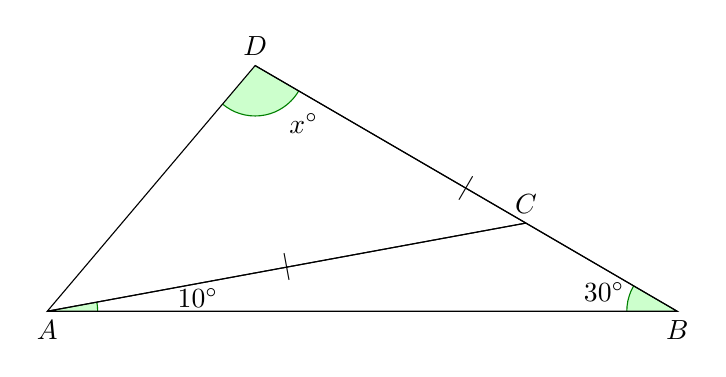
\begin{tikzpicture}[x=\figuresize,y=\figuresize]
	\coordinate [label=below:$A$] (A) at (0,0);
	\coordinate [label=below:$B$] (B) at (1,0);
	\coordinate [label=above:$C$] (C) at (0.76,0.14);
	\coordinate [label=above:$D$] (D) at (0.33,0.39);
	
	\makeangle{C}{A}{B}{10}{0.08}{5}{0.24}
	\makeangle{A}{B}{C}{30}{0.08}{165}{0.12}
	\makeangle{A}{D}{B}{x}{0.08}{310}{0.12}

	\draw (A) -- (B) -- (C) -- (A) -- (D) -- (C);
	\draw (A) -- node[sloped] {$|$} (C);
	\draw (B) -- node[sloped] {$|$} (D);

	\end{tikzpicture}
	\caption{$\overline{DB} = \overline{AC}; \angle \hat{CAB} = 10\degree; \angle \hat{ABD} = 30\degree; \angle \hat{ADB} = x\degree$}
\end{figure}

\subsection{Solution 1}

\begin{figure}
	\centering
	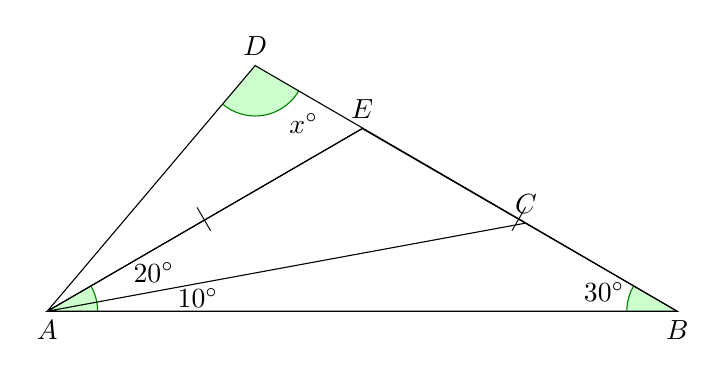
\begin{tikzpicture}[x=\figuresize,y=\figuresize]
	\coordinate [label=below:$A$] (A) at (0,0);
	\coordinate [label=below:$B$] (B) at (1,0);
	\coordinate [label=above:$C$] (C) at (0.76,0.14);
	\coordinate [label=above:$D$] (D) at (0.33,0.39);
	\coordinate [label=above:$E$] (E) at (0.5,0.29);
	
	\makeangle{C}{A}{B}{10}{0.08}{5}{0.24}
	\makeangle{A}{B}{C}{30}{0.08}{165}{0.12}
	\makeangle{A}{D}{B}{x}{0.08}{310}{0.12}
	\makeangle{E}{A}{C}{20}{0.08}{20}{0.18}

	\draw (E) -- (A) -- (B) -- (C) -- (A) -- (D) -- (C);
	\draw (A) -- node[sloped] {$|$} (E) -- node[sloped] {$|$} (B);

	\end{tikzpicture}
	\caption{$\angle \hat{EAC} = 20\degree; \angle hat{EAB} = \angle \hat{EBA} \therefore \overline{AE} = \overline{EB}$}
\end{figure}

\begin{figure}
	\centering
	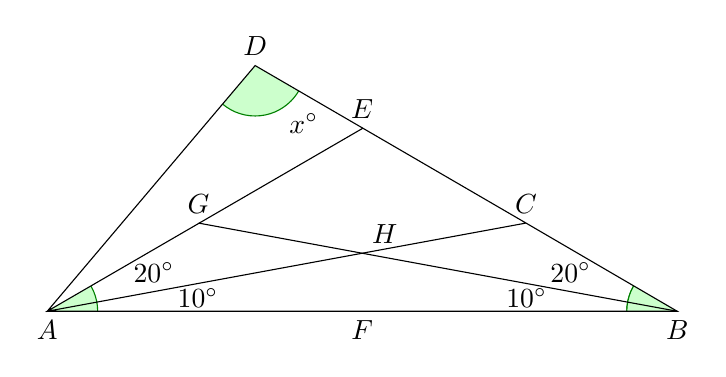
\begin{tikzpicture}[x=\figuresize,y=\figuresize]
	\coordinate [label=below:$A$] (A) at (0,0);
	\coordinate [label=below:$B$] (B) at (1,0);
	\coordinate [label=above:$C$] (C) at (0.76,0.14);
	\coordinate [label=above:$D$] (D) at (0.33,0.39);
	\coordinate [label=above:$E$] (E) at (0.5,0.29);
	\coordinate [label=below:$F$] (F) at (0.5,0);
	\coordinate [label=above:$G$] (G) at (0.24,0.14);
	\coordinate [label=above right:$H$] (H) at (0.5,0.092);
	
	\makeangle{C}{A}{B}{10}{0.08}{5}{0.24}
	\makeangle{A}{B}{C}{20}{0.08}{160}{0.18}
	\makeangle{A}{B}{C}{10}{0.08}{175}{0.24}
	\makeangle{A}{D}{B}{x}{0.08}{310}{0.12}
	\makeangle{E}{A}{C}{20}{0.08}{20}{0.18}

	\draw (E) -- (A) -- (B) -- (C) -- (A) -- (D) -- (C);
	\draw (B) -- (G);

	\end{tikzpicture}
	\caption{$\angle \hat{GBA} = 10\degree; \overline{GB} = \overline{AC}$}
\end{figure}

\begin{figure}
	\centering
	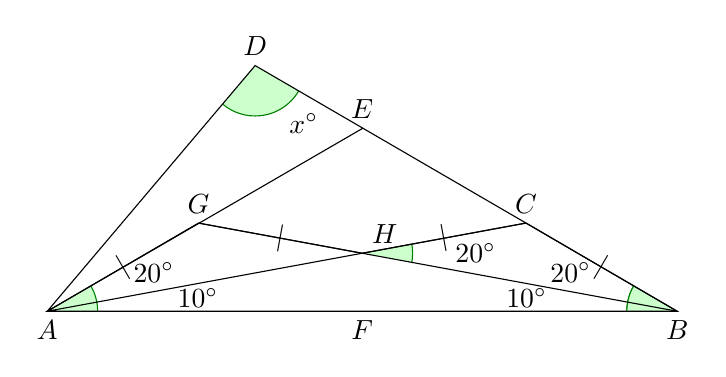
\begin{tikzpicture}[x=\figuresize,y=\figuresize]
	\coordinate [label=below:$A$] (A) at (0,0);
	\coordinate [label=below:$B$] (B) at (1,0);
	\coordinate [label=above:$C$] (C) at (0.76,0.14);
	\coordinate [label=above:$D$] (D) at (0.33,0.39);
	\coordinate [label=above:$E$] (E) at (0.5,0.29);
	\coordinate [label=below:$F$] (F) at (0.5,0);
	\coordinate [label=above:$G$] (G) at (0.24,0.14);
	\coordinate [label=above right:$H$] (H) at (0.5,0.092);
	
	\makeangle{C}{A}{B}{10}{0.08}{5}{0.24}
	\makeangle{A}{B}{C}{20}{0.08}{160}{0.18}
	\makeangle{A}{B}{C}{10}{0.08}{175}{0.24}
	\makeangle{A}{D}{B}{x}{0.08}{310}{0.12}
	\makeangle{E}{A}{C}{20}{0.08}{20}{0.18}
	\makeangle{C}{H}{B}{20}{0.08}{0}{0.18}

	\draw (E) -- (A) -- (B) -- (C) -- (A) -- (D) -- (C);
	\draw (B) -- (G);
	\draw (A) -- node[sloped] {$|$}
		(G) -- node[sloped] {$|$}
		(H) -- node[sloped] {$|$}
		(C) -- node[sloped] {$|$} (B);

	\end{tikzpicture}
	\caption{$\angle \hat{HAB} + \angle \hat{HBA} = \angle \hat{CHB} = \angle \hat{GHA} = 20\degree$}
\end{figure}

\begin{figure}
	\centering
	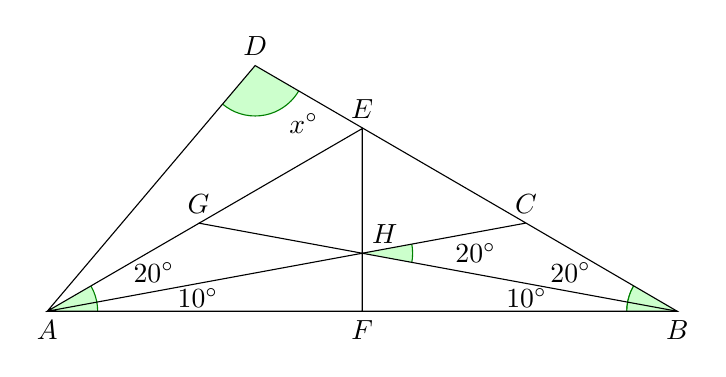
\begin{tikzpicture}[x=\figuresize,y=\figuresize]
	\coordinate [label=below:$A$] (A) at (0,0);
	\coordinate [label=below:$B$] (B) at (1,0);
	\coordinate [label=above:$C$] (C) at (0.76,0.14);
	\coordinate [label=above:$D$] (D) at (0.33,0.39);
	\coordinate [label=above:$E$] (E) at (0.5,0.29);
	\coordinate [label=below:$F$] (F) at (0.5,0);
	\coordinate [label=above:$G$] (G) at (0.24,0.14);
	\coordinate [label=above right:$H$] (H) at (0.5,0.092);
	
	\makeangle{C}{A}{B}{10}{0.08}{5}{0.24}
	\makeangle{A}{B}{C}{20}{0.08}{160}{0.18}
	\makeangle{A}{B}{C}{10}{0.08}{175}{0.24}
	\makeangle{A}{D}{B}{x}{0.08}{310}{0.12}
	\makeangle{E}{A}{C}{20}{0.08}{20}{0.18}
	\makeangle{C}{H}{B}{20}{0.08}{0}{0.18}

	\draw (F) -- (E) -- (A) -- (B) -- (C) -- (A) -- (D) -- (C);
	\draw (B) -- (G);

	\end{tikzpicture}
	\caption{$\overline{EF} \perp \overline{AB}; \angle \hat{EFB} = \angle \hat{EFA} = 90\degree; \triangle AEF \equiv \triangle BEF$}
\end{figure}

\begin{figure}
	\centering
	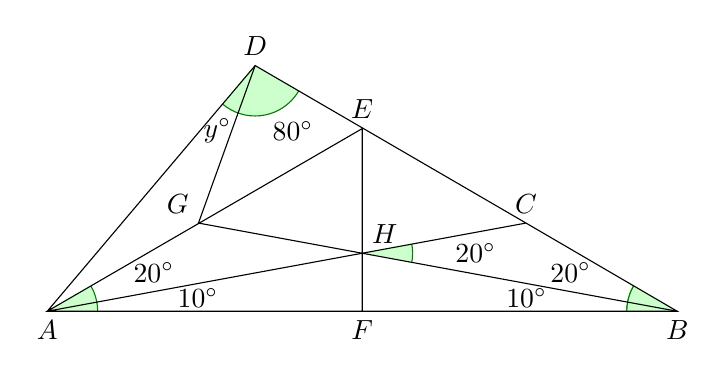
\begin{tikzpicture}[x=\figuresize,y=\figuresize]
	\coordinate [label=below:$A$] (A) at (0,0);
	\coordinate [label=below:$B$] (B) at (1,0);
	\coordinate [label=above:$C$] (C) at (0.76,0.14);
	\coordinate [label=above:$D$] (D) at (0.33,0.39);
	\coordinate [label=above:$E$] (E) at (0.5,0.29);
	\coordinate [label=below:$F$] (F) at (0.5,0);
	\coordinate [label=above left:$G$] (G) at (0.24,0.14);
	\coordinate [label=above right:$H$] (H) at (0.5,0.092);
	
	\makeangle{C}{A}{B}{10}{0.08}{5}{0.24}
	\makeangle{A}{B}{C}{20}{0.08}{160}{0.18}
	\makeangle{A}{B}{C}{10}{0.08}{175}{0.24}
	\makeangle{E}{A}{C}{20}{0.08}{20}{0.18}
	\makeangle{A}{D}{G}{y}{0.08}{240}{0.12}
	\makeangle{C}{H}{B}{20}{0.08}{0}{0.18}
	\makeangle{B}{D}{G}{80}{0.08}{300}{0.12}

	\draw (F) -- (E) -- (A) -- (B) -- (C) -- (A) -- (D) -- (C);
	\draw (B) -- (G) -- (D);

	\end{tikzpicture}
	\caption{$\overline{BG} = \overline{BD} \therefore \angle \hat{DGB} = 80\degree; \angle \hat{GAH} = \angle \hat{GHA} = 20\degree \therefore \angle \hat{EGH} = 40\degree \therefore \angle \hat{DGE} = 40\degree$}
\end{figure}

\begin{figure}
	\centering
	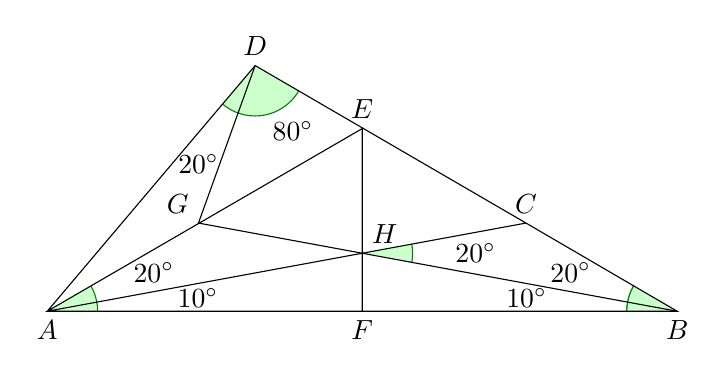
\begin{tikzpicture}[x=\figuresize,y=\figuresize]
	\coordinate [label=below:$A$] (A) at (0,0);
	\coordinate [label=below:$B$] (B) at (1,0);
	\coordinate [label=above:$C$] (C) at (0.76,0.14);
	\coordinate [label=above:$D$] (D) at (0.33,0.39);
	\coordinate [label=above:$E$] (E) at (0.5,0.29);
	\coordinate [label=below:$F$] (F) at (0.5,0);
	\coordinate [label=above left:$G$] (G) at (0.24,0.14);
	\coordinate [label=above right:$H$] (H) at (0.5,0.092);
	
	\makeangle{C}{A}{B}{10}{0.08}{5}{0.24}
	\makeangle{A}{B}{C}{20}{0.08}{160}{0.18}
	\makeangle{A}{B}{C}{10}{0.08}{175}{0.24}
	\makeangle{E}{A}{C}{20}{0.08}{20}{0.18}
	\makeangle{A}{D}{G}{20}{0.08}{240}{0.18}
	\makeangle{B}{D}{G}{80}{0.08}{300}{0.12}
	\makeangle{C}{H}{B}{20}{0.08}{0}{0.18}

	\draw (F) -- (E) -- (A) -- (B) -- (C) -- (A) -- (D) -- (C);
	\draw (B) -- (G) -- (D);

	\end{tikzpicture}
	\caption{$\angle \hat{DGE} = \angle \hat{HGE} = 40\degree and \angle \hat{EDG} = \angle \hat{EHG} = 80\degree \therefore \triangle DEG = \triangle HEG \therefore \overline{DG} = \overline{HG} = \overline{AG} \therefore \angle \hat{DAG} = \angle \hat{ADG} = 20\degree$}
\end{figure}

    \section{Triangulo Russo}

\subsection{Problem}

\begin{figure}[ht]
	\centering
	\begin{tikzpicture}[x=\figuresize,y=\figuresize]
	\coordinate [label=below:$A$] (A) at (0,0);
	\coordinate [label=below:$B$] (B) at (1,0);
	\coordinate [label=above:$C$] (C) at (0.5,2.83);
	\coordinate [label=above left:$D$] (D) at (0.17,0.98);
	\coordinate [label=below right:$E$] (E) at (0.765,1.33);
	
	\makeangle{C}{A}{E}{20}{0.08}{70}{0.30}
	\makeangle{B}{A}{E}{60}{0.08}{30}{0.12}
	\makeangle{A}{B}{D}{50}{0.08}{155}{0.12}
	\makeangle{D}{B}{E}{30}{0.08}{110}{0.18}
	\makeangle{D}{E}{A}{x}{0.08}{225}{0.18}

	\draw (A) -- (B) -- (C) -- cycle;
	\draw (B) -- (D) -- (E) -- (A);

	\end{tikzpicture}
	\caption{$\angle \hat{DAE} = 20\degree; \angle \hat{EAB} = 60\degree; \angle \hat{DBA} = 50\degree; \angle \hat{CBD} = 30\degree$}
\end{figure}

\subsection{Solution 1}

\begin{figure}
	\centering
	\begin{tikzpicture}[x=\figuresize,y=\figuresize]
	\coordinate [label=below:$A$] (A) at (0,0);
	\coordinate [label=below:$B$] (B) at (1,0);
	\coordinate [label=above:$C$] (C) at (0.5,2.83);
	\coordinate [label=above left:$D$] (D) at (0.17,0.98);
	\coordinate [label=below right:$E$] (E) at (0.765,1.33);
	\coordinate [label=above left:$F$] (F) at (-0.27,1.51);
	\coordinate (Z) at (-0.40,1.28);
	
	\makeangle{C}{A}{E}{20}{0.08}{70}{0.30}
	\makeangle{B}{A}{E}{60}{0.08}{30}{0.12}
	\makeangle{A}{B}{D}{50}{0.08}{155}{0.12}
	\makeangle{D}{B}{E}{30}{0.08}{110}{0.18}
	\makeangle{A}{C}{B}{20}{0.08}{270}{0.30}
	\makeangle{A}{C}{F}{20}{0.08}{250}{0.30}

	\draw (A) -- (B) -- (C) -- cycle;
	\draw (B) -- (D) -- (E) -- (A);
	\draw (E) -- node[sloped] {$|$}
		(C) -- node[sloped] {$|$}
		(F) -- (Z);

	\end{tikzpicture}
	\caption{$\angle \hat{FCD} = 20\degree; \overline{CF} = \overline{CE}; \overline{FC} \parallel \overline{AE}$}
\end{figure}

\begin{figure}
	\centering
	\begin{tikzpicture}[x=\figuresize,y=\figuresize]
	\coordinate [label=below:$A$] (A) at (0,0);
	\coordinate [label=below:$B$] (B) at (1,0);
	\coordinate [label=above:$C$] (C) at (0.5,2.83);
		\coordinate [label=below left:$D$] (D) at (0.17,0.98);
	\coordinate [label=below right:$E$] (E) at (0.765,1.33);
	\coordinate [label=above left:$F$] (F) at (-0.27,1.51);
	\coordinate (Z) at (-0.40,1.28);
	
	\makeangle{C}{A}{E}{20}{0.08}{70}{0.30}
	\makeangle{B}{A}{E}{60}{0.08}{30}{0.12}
	\makeangle{A}{B}{D}{50}{0.08}{155}{0.12}
	\makeangle{D}{B}{E}{30}{0.08}{110}{0.18}
	\makeangle{A}{C}{B}{20}{0.08}{270}{0.30}
	\makeangle{A}{C}{F}{20}{0.08}{250}{0.30}
	\makeangle{C}{F}{D}{110}{0.08}{5}{0.18}

	\draw (A) -- (B) -- (C) -- cycle;
	\draw (B) -- (D) -- (E) -- (A);
	\draw (E) -- (C) -- (F) -- (D);
	\draw (F) -- (Z);


	\end{tikzpicture}
	\caption{$F \in \overline{BD}$}
\end{figure}

\begin{figure}
	\centering
	\begin{tikzpicture}[x=\figuresize,y=\figuresize]
	\coordinate [label=below:$A$] (A) at (0,0);
	\coordinate [label=below:$B$] (B) at (1,0);
	\coordinate [label=above:$C$] (C) at (0.5,2.83);
		\coordinate [label=below left:$D$] (D) at (0.17,0.98);
	\coordinate [label=below right:$E$] (E) at (0.765,1.33);
	\coordinate [label=above left:$F$] (F) at (-0.27,1.51);
	\coordinate (Z) at (-0.40,1.28);
	
	\makeangle{C}{A}{E}{20}{0.08}{70}{0.30}
	\makeangle{B}{A}{E}{60}{0.08}{30}{0.12}
	\makeangle{A}{B}{D}{50}{0.08}{155}{0.12}
	\makeangle{D}{B}{E}{30}{0.08}{110}{0.18}
	\makeangle{A}{C}{B}{20}{0.08}{270}{0.30}
	\makeangle{A}{C}{F}{20}{0.08}{250}{0.30}
	\makeangle{C}{F}{D}{110}{0.08}{5}{0.18}
	\makeangle{A}{F}{D}{30}{0.08}{295}{0.24}
	\makeangle{F}{A}{D}{20}{0.08}{90}{0.24}

	\draw (A) -- (B) -- (C) -- cycle;
	\draw (B) -- (D) -- (E) -- (A);
	\draw (E) -- (C) -- (F) -- (D);
	\draw (A) -- (F) -- (Z);


	\end{tikzpicture}
	\caption{$\triangle CDB \approx \triangle ADF \therefore \angle \hat{CAF} = \hat{ACE}; \angle \hat{CBF} = \angle \hat{BFA}$}
\end{figure}

\begin{figure}
	\centering
	\begin{tikzpicture}[x=\figuresize,y=\figuresize]
	\coordinate [label=below:$A$] (A) at (0,0);
	\coordinate [label=below:$B$] (B) at (1,0);
	\coordinate [label=above:$C$] (C) at (0.5,2.83);
		\coordinate [label=below left:$D$] (D) at (0.17,0.98);
	\coordinate [label=below right:$E$] (E) at (0.765,1.33);
	\coordinate [label=above left:$F$] (F) at (-0.27,1.51);
	\coordinate [label=above right:$G$] (G) at (0.25,1.42);
	\coordinate (Z) at (-0.40,1.28);
	
	\makeangle{C}{A}{E}{20}{0.08}{70}{0.30}
	\makeangle{B}{A}{E}{60}{0.08}{30}{0.12}
	\makeangle{A}{B}{D}{50}{0.08}{155}{0.12}
	\makeangle{D}{B}{E}{30}{0.08}{110}{0.18}
	\makeangle{A}{C}{B}{20}{0.08}{270}{0.30}
	\makeangle{A}{C}{F}{20}{0.08}{250}{0.30}
	\makeangle{E}{F}{D}{40}{0.08}{330}{0.18}
	\makeangle{C}{F}{E}{70}{0.08}{25}{0.18}
	\makeangle{A}{F}{D}{30}{0.08}{295}{0.24}
	\makeangle{F}{A}{D}{20}{0.08}{90}{0.24}

	\makeangle{D}{E}{G}{40}{0.08}{190}{0.18}
	\makeangle{A}{E}{D}{30}{0.08}{225}{0.24}

	\draw (A) -- (B) -- (C) -- cycle;
	\draw (B) -- (D) -- (E) -- (A);
	\draw (F) -- (G) -- (E) -- (C) -- (F) -- (D);
	\draw (A) -- (F) -- (Z);


	\end{tikzpicture}
	\caption{$\triangle FGD \equiv \triangle EGD \therefore \angle \hat{GED} = 40\degree \therefore \angle \hat{DEA} = 30\degree$}
\end{figure}

\subsection{Solution 2}

\begin{figure}[ht]
	\centering
	\begin{tikzpicture}[x=\figuresize,y=\figuresize]
	\coordinate [label=below:$A$] (A) at (0,0);
	\coordinate [label=below:$B$] (B) at (1,0);
	\coordinate [label=above:$C$] (C) at (0.5,2.83);
	\coordinate [label=above left:$D$] (D) at (0.17,0.98);
	\coordinate [label=below right:$E$] (E) at (0.765,1.33);
	\coordinate [label=right:$F$] (F) at (0.94,0.34);
	
	\makeangle{C}{A}{E}{20}{0.08}{70}{0.30}
	\makeangle{B}{A}{F}{20}{0.08}{10}{0.24}
	\makeangle{F}{A}{E}{40}{0.08}{40}{0.18}
	\makeangle{A}{B}{D}{50}{0.08}{155}{0.12}
	\makeangle{D}{B}{E}{30}{0.08}{110}{0.18}

	\draw (A) -- (B) -- (C) -- cycle;
	\draw (B) -- (D) -- (E) -- (A) -- (F);

	\end{tikzpicture}
	\caption{$\overline{AD} = \overline{AB} = \overline{AF}; \angle \hat{FAB} = 20\degree; \angle \hat{EAF} = 40\degree$}
\end{figure}

\begin{figure}
	\centering
	\begin{tikzpicture}[x=\figuresize,y=\figuresize]
	\coordinate [label=below:$A$] (A) at (0,0);
	\coordinate [label=below:$B$] (B) at (1,0);
	\coordinate [label=above:$C$] (C) at (0.5,2.83);
	\coordinate [label=above left:$D$] (D) at (0.17,0.98);
	\coordinate [label=below right:$E$] (E) at (0.765,1.33);
	\coordinate [label=right:$F$] (F) at (0.94,0.34);
	
	\makeangle{C}{A}{E}{20}{0.08}{70}{0.30}
	\makeangle{B}{A}{F}{20}{0.08}{10}{0.24}
	\makeangle{F}{A}{E}{40}{0.08}{40}{0.18}
	\makeangle{A}{B}{D}{50}{0.08}{155}{0.12}
	\makeangle{D}{B}{E}{30}{0.08}{110}{0.18}
	\makeangle{D}{F}{A}{60}{0.08}{170}{0.18}
	\makeangle{A}{D}{F}{60}{0.08}{290}{0.18}

	\draw (A) -- (B) -- (C) -- cycle;
	\draw (B) -- (D) -- (E) -- (A) -- (F) -- (D);
	\draw (D) -- node[sloped] {$|$}
		(F) -- node[sloped] {$|$}
		(A) -- node[sloped] {$|$} (D);

	\end{tikzpicture}
	\caption{$\overline{DA} = \overline{AF} = \overline{FD}$}
\end{figure}

\begin{figure}
	\centering
	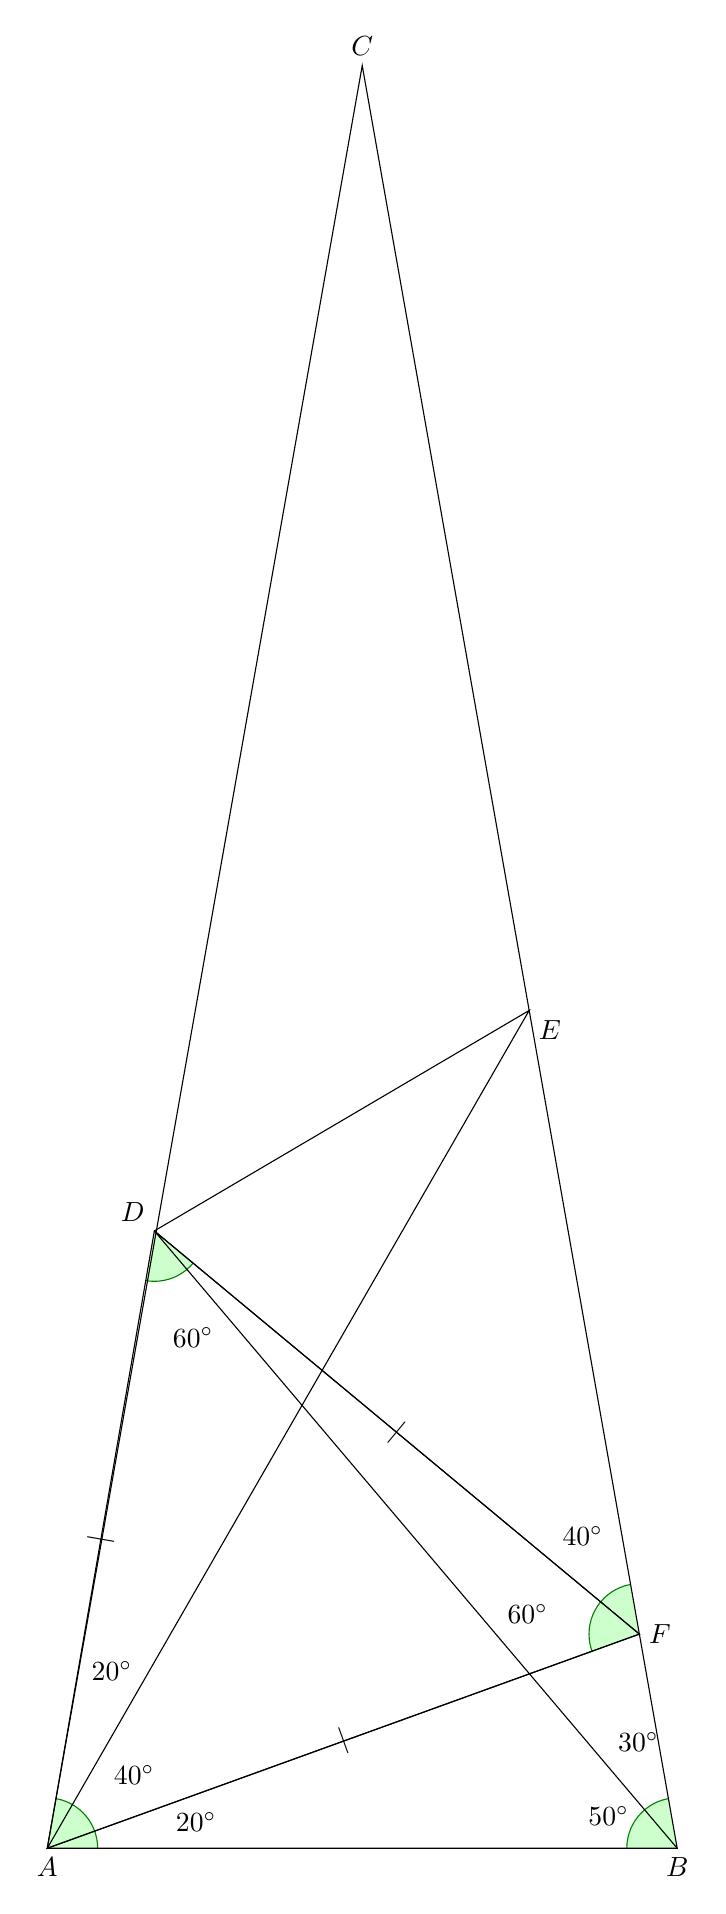
\begin{tikzpicture}[x=\figuresize,y=\figuresize]
	\coordinate [label=below:$A$] (A) at (0,0);
	\coordinate [label=below:$B$] (B) at (1,0);
	\coordinate [label=above:$C$] (C) at (0.5,2.83);
	\coordinate [label=above left:$D$] (D) at (0.17,0.98);
	\coordinate [label=below right:$E$] (E) at (0.765,1.33);
	\coordinate [label=right:$F$] (F) at (0.94,0.34);
	
	\makeangle{C}{A}{E}{20}{0.08}{70}{0.30}
	\makeangle{B}{A}{F}{20}{0.08}{10}{0.24}
	\makeangle{F}{A}{E}{40}{0.08}{40}{0.18}
	\makeangle{A}{B}{D}{50}{0.08}{155}{0.12}
	\makeangle{D}{B}{E}{30}{0.08}{110}{0.18}
	\makeangle{D}{F}{A}{60}{0.08}{170}{0.18}
	\makeangle{A}{D}{F}{60}{0.08}{290}{0.18}
	\makeangle{E}{F}{D}{40}{0.08}{120}{0.18}

	\draw (A) -- (B) -- (C) -- cycle;
	\draw (B) -- (D) -- (E) -- (A) -- (F) -- (D);
	\draw (D) -- node[sloped] {$|$}
		(F) -- node[sloped] {$|$}
		(A) -- node[sloped] {$|$} (D);

	\end{tikzpicture}
	\caption{$\overline{DA} = \overline{AF} = \overline{FD} \therefore \angle \hat{DFE} = 40\degree$}
\end{figure}

\begin{figure}
	\centering
	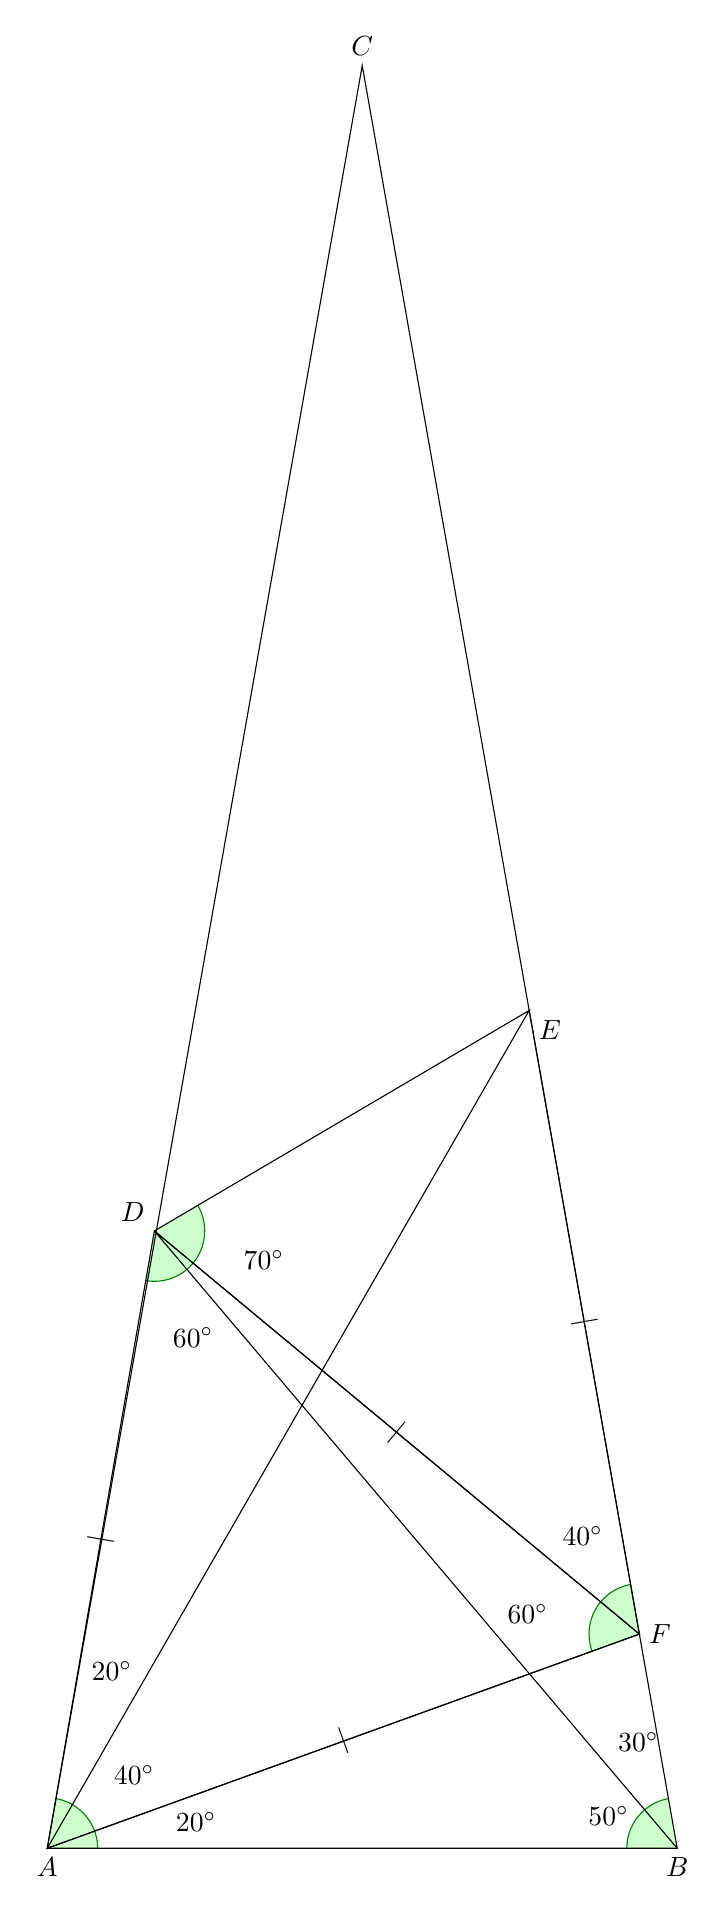
\begin{tikzpicture}[x=\figuresize,y=\figuresize]
	\coordinate [label=below:$A$] (A) at (0,0);
	\coordinate [label=below:$B$] (B) at (1,0);
	\coordinate [label=above:$C$] (C) at (0.5,2.83);
	\coordinate [label=above left:$D$] (D) at (0.17,0.98);
	\coordinate [label=below right:$E$] (E) at (0.765,1.33);
	\coordinate [label=right:$F$] (F) at (0.94,0.34);
	
	\makeangle{C}{A}{E}{20}{0.08}{70}{0.30}
	\makeangle{B}{A}{F}{20}{0.08}{10}{0.24}
	\makeangle{F}{A}{E}{40}{0.08}{40}{0.18}
	\makeangle{A}{B}{D}{50}{0.08}{155}{0.12}
	\makeangle{D}{B}{E}{30}{0.08}{110}{0.18}
	\makeangle{D}{F}{A}{60}{0.08}{170}{0.18}
	\makeangle{A}{D}{F}{60}{0.08}{290}{0.18}
	\makeangle{E}{F}{D}{40}{0.08}{120}{0.18}
	\makeangle{F}{D}{E}{70}{0.08}{345}{0.18}

	\draw (A) -- (B) -- (C) -- cycle;
	\draw (B) -- (D) -- (E) -- (A) -- (F) -- (D);
	\draw (D) -- node[sloped] {$|$}
		(F) -- node[sloped] {$|$}
		(A) -- node[sloped] {$|$} (D);
	\draw (E) -- node[sloped] {$|$} (F);

	\end{tikzpicture}
	\caption{$\angle \hat{AFE} = 40\degree \therefore \overline{EF} = \overline{DF} \therefore \angle \hat{FDE} = \angle \hat{FED} = 70\degree$}
\end{figure}


\end{document}
